\documentclass[a4paper,11pt]{report}
\usepackage{geometry}\geometry{a4paper,top=3.5cm,bottom=3.5cm,%
left=2.5cm,right=2.5cm,heightrounded,bindingoffset=0mm}
\usepackage[T1]{fontenc}
\usepackage[utf8]{inputenc}
\usepackage[italian]{babel}
\usepackage{graphicx}
\usepackage[table,xcdraw]{xcolor}
\usepackage{subfig}
\usepackage{amsmath,amsfonts,amssymb,braket,mathrsfs,eurosym}
\usepackage{float}
\usepackage{tabularx,booktabs,multirow}
\usepackage{lscape}
\usepackage{longtable}
\usepackage[output-decimal-marker={,}]{siunitx}
\usepackage{pdfpages}
%\usepackage{minipage}
\usepackage{tikz}
\usepackage{xspace}% per lo spazio intelligente
\newcommand{\e}{\`E\xspace}  %E'
\newcommand{\teuro}{\text{\euro}}%il simbolo dell'euro dentro le formula matematiche diventa "e". con \text diventa €
\newcommand{\red}[1]{\textcolor{red}{#1}}
\newcommand{\omissis}{[\textellipsis\unkern]} %puntini di sospensione
\newcommand{\xlam}{\hbox{X-LAM}} %per non far andare a capo XLAM dopo il trattino
%Ci va un {} nel casso di spazio dopo omiss o xlam. Non ci va se dopo c'è un punto.
\usepackage{quoting}
\quotingsetup{font=small}
\usepackage{caption}
\captionsetup{tableposition=top,figureposition=bottom,font=small}\captionsetup{format=hang,labelfont={bf}}
\usepackage{plain}
\usepackage{epsfig}
\usepackage{titlesec} % per formato custom dei titoli dei capitoli
\usepackage{hyperref}
%\usepackage[style=numeric-comp]{biblatex}
\usepackage[autostyle,italian=guillemets]{csquotes}
%numeric: la bibliografia ha i numeri
%backref: indica nella bibliografia le pagine in cui ci sono le citazioni
\usepackage[style=numeric,backend=biber,backref,hyperref]{biblatex}
\addbibresource{Bibliografia.bib}
%\usepackage{appendix}
\begin{document}
% Fa schifo lo so, ma deriva dal template messo a disposizione dal DISI di unitn un po' rielaborato
% Un giorno userò la classe frontespizio 

%Il counter pagina è settato nel main dopo il TOC 
\pagestyle{plain}
\thispagestyle{empty}
\begin{center}
  \begin{figure}[H]
    \centerline{
\psfig{file=img/logo_unitn_black_center.eps,
                        width=0.8\textwidth,trim = 0 0.9cm 0 0.5cm}}
  \end{figure}
\line(1,0){450}

  \Large\textsc{Dipartimento di Ingegneria Civile, Ambientale e Meccanica\\}
  \Large{Corso di Laurea in Ingegneria Civile
  }

  \vspace{2.7 cm} 
  %\Large\textsc{Elaborato finale\\} 
  %\vspace{1 cm} 
  \Huge\textsc{relazione di programmazione costi e contabilità dei lavori\\}
  
  \vspace{0.5 cm}
  \Large{\it{Analisi di un edificio volta a trovare i materiali economicamente più vantaggiosi per la costruzione di pareti e solai}}


  \vspace{3 cm} 
  \begin{tabular*}{\textwidth}{ l @{\extracolsep{\fill}} r }
  \Large\textsc{Docente} & \Large\textsc{Studenti}\\
  \Large{Mario Claudio Dejaco}& \Large{Stefano Bernardi 188638}\\
  	 & \Large{Anna Boso 179794}\\
  	 & \Large{Angelica Lenzi 173852}\\
  	 & \Large{Nicola Meoli 186100}\\
  	 & \Large{Mirko Vindimian 185076}\\
  	 & \Large{Luca Zorzi 185098}\\
  	
  \end{tabular*}

  \vspace{2.1cm} 
    \line(1,0){450}
    
  \Large{Anno accademico 2018/19}
  
\end{center}


\tableofcontents
%\setcounter{page}{1}
%Tabelle e figure sulla stessa pagina:
%Le aggiunge all'indice. phantomsection serve per non far casini con hyperref
\clearpage
\begingroup
   %\let\cleardoublepage\relax  % book
    \let\clearpage\relax        % report
        \listoftables
        \phantomsection
        \addcontentsline{toc}{chapter}{Elenco delle tabelle}
        %
        \listoffigures
        \phantomsection
        \addcontentsline{toc}{chapter}{Elenco delle figure}
\endgroup
%\thispagestyle{empty}
% redefinizione del formato del titolo del capitolo
      % da formato
      %   Capitolo X
      %   Titolo capitolo
      % a formato
      %   X   Titolo capitolo 
	\titleformat{\chapter}
        {\normalfont\Huge\bfseries}{\thechapter}{1em}{}
	\titlespacing*{\chapter}{0pt}{0in}{0.02in}
	\titlespacing*{\section}{0pt}{0.2in}{0.02in}
	\titlespacing*{\subsection}{0pt}{0.10in}{0.02in}
%%%%%%%%%%%%%%%%%%%%%%%%%%%%%%%%%%%%%%%%%%%%%%%%%%%%%%%%%%%%
%%%%%%%%%%%%%%%%%%%%%%%%%%%%%%%%%%%%%%%%%%%%%%%%%%%%%%%%%%%%
%    
%bibliografia
%\nocite{mcgraw}%senza un preciso punto nel testo
%\bibliographystyle{plain}
\cleardoublepage
\phantomsection
\printbibliography[heading=bibintoc]
%Capitoli introduttivi
    \chapter{Introduzione dell'analisi svolta}
Con questa relazione si riporta un'analisi economica di un edificio scelto, nella quale si è cercato di trovare i materiali da costruzione economicamente più vantaggiosi per la sua costruzione.
\section{Stato zero edificio scelto}
Come prima cosa si è scelto un edificio nel quale si avesse una certa quantità di documentazione da riuscire a trarne un computo metrico degli elementi.
\e stato quindi utilizzato un progetto di cinque villette a schiera, il quale, per l'occasione, è stato collocato in una specifica zona di Trento, in modo da poter ricavare i valori immobiliari della zona. 
Zonizzazione che è riportata nelle pagine \pageref{Edificio} e successive.

Sono stati scelti dei vincoli obbligatori da dover rispettare, inderogabili a seconda delle varie ipotesi successive. 
Tali vincoli rappresentano la dimensione tra gli interassi delle villette a schiera -- non doveva variare in base ai materiali scelti -- e la trasmittanza termica delle pareti esterne. 

Il progetto di partenza, riportato negli allegati a pagina \pageref{piante}, prevedeva un pacchetto della muratura esterna composto da: parete portante in laterizio, isolante in lana di roccia e intonaco esterno generico. Come solaio intermedio e di copertura una struttura in laterocemento.
Queste caratteristiche dei materiali compongono lo stato zero dell'edificio, e sono state usate come paragone rispetto gli altri materiali.

Questo stesso progetto è stato scomposto utilizzando la Tabella 21 delle \emph{OmniClass 2012}. 
Tale operazione, riportata nella WBS a pagina \pageref{WBS}, è servita per capire quali elementi variassero in base ai materiali scelti.
Le componenti uguali tra le varie opzioni, come si vedrà, non sono state analizzate in quanto non producevano differenze di costi.
\section{Descrizione del procedimento utilizzato per l'analisi}
Per valutare quali materiali fossero più vantaggiosi per la costruzione delle cinque villette a schiera, si è suddiviso il problema in più parti.
Si è partiti analizzando le parete perimetrali dell'intero edificio e definendo una stratigrafia della parete composta da tre macro categorie: struttura, isolante e rivestimento esterno.
Per queste tre categorie sono state fatte varie ipotesi di possibili materiali e per ciascuna di esse è stato trovato quello migliore, valutandone diversi aspetti. 
Per ogni materiale è stato valutato il costo ad opera conclusa utilizzando il prezzario della Provincia di Trento e -- dove ce ne fosse bisogno -- facendo un'analisi dei prezzi utilizzando i dati messi a disposizione dalle aziende produttrici.
In base alla tipologia del materiale sono stati presi in considerazione vari parametri come lo spessore, la manutenzione o la tempistica di messa in opera.

Si è continuata l'analisi concentrandosi solo sulla  struttura e valutando solamente le pareti interne, il solaio intermedio e quello di copertura.
Sono stati presi in considerazione il materiale vincente della precedente fase e quello della struttura zero di partenza.
Ovviamente si è fatto in modo che pareti e solai avessero una certa continuità e fossero quindi compatibili tra loro.

Come ultima fase sono state fatte delle considerazioni sui due materiali per cercare di trovare una motivazione a propendere per uno o l'altro, nonostante i costi maggiori. 

Nei prossimi capitoli verrà spiegato nel dettaglio l'analisi in ogni sua parte e verranno riportate le relative tabelle di confronto con i rispettivi computi.

Per non appesantire troppo il testo, alcune tabelle e alcuni documenti di contorno, sono stati riportati in fondo a questa relazione e citati, quando necessario, all'interno del testo.
%Capitoli analisi pareti esterne
    \chapter{Analisi delle pareti esterne}
Sono stati scelti vari materiali e che verranno riportati nei paragrafi successivi con un'apposita descrizione.  
Come si vedrà in seguito, per ogni categoria sono stati valutati aspetti diversi, in quanto in alcuni casi diventavano del tutto trascurabili e alla pari tra i contendenti.

Come prima cosa è stata fatta un'analisi del valore per tutti i materiali in modo da riuscire ad avere un termine di confronto tra i materiali con diversi costi ma con proprietà molto diverse. 
Nell'analisi del valore riportata a pagina \pageref{fig:AnalisiValore} sono stati utilizzati i criteri che vengono riportati nella norma \textsc{UNI 829-2:1983}.
Per ogni criterio è stato assegnato un punteggio da 1 a 5  e utilizzando le caratteristiche riportate dalle aziende produttrici o dall'esperienza. 
Infine si è trovato il totale sommandoli. 
Come risulterà dalle analisi che verranno ora riportate, i maggiori punteggi ottenuti da ciascun materiale, corrispondono anche ai maggiori costi di essi.
Per alcuni risulterà talmente maggiore da non consentire nemmeno di poter fare un'analisi più approfondita.

Si elencano ora i diversi criteri che sono stati tenuti in conto.
Per tutte le categorie è stato calcolato il costo del materiale, preso da prezzario o da analisi prezzi.
A seconda dell'incidenza sono state prese come termine di paragone tempo di posa, manutenzione e spessore risparmiato.
Per quanto riguarda il tempo di posa i dati sono stati ottenuti dal tempario \textcite{grosso2007tempario} e convertiti in euro utilizzando il prezzo unitario dell'operaio (comune o specializzato). 
Nel caso del rivestimento è stato necessario elaborare un piano di manutenzione, come si vedrà in seguito. 
In questo caso è stato valutato come molto incidente i costi che si avranno successivamente alla costruzione dell'edificio.
Lo spessore minore di alcuni strati è stato utilizzato per calcolare la superficie libera risparmiata rispetto alla soluzione zero. 
Si è supposto poi di poter recuperare dei soldi da tale superficie vendendola o affittandola.
Sono stati presi i valori analizzando i prezzi di mercato forniti dall'Agenzia delle Entrate a Trento e ottenendo così un  prezzo di vendita di \SI{3000}{\teuro / \square\metre} e di di affitto di \SI{10.41}{\teuro /\square\metre mese }.


\begin{figure}[p]
    \centering 
    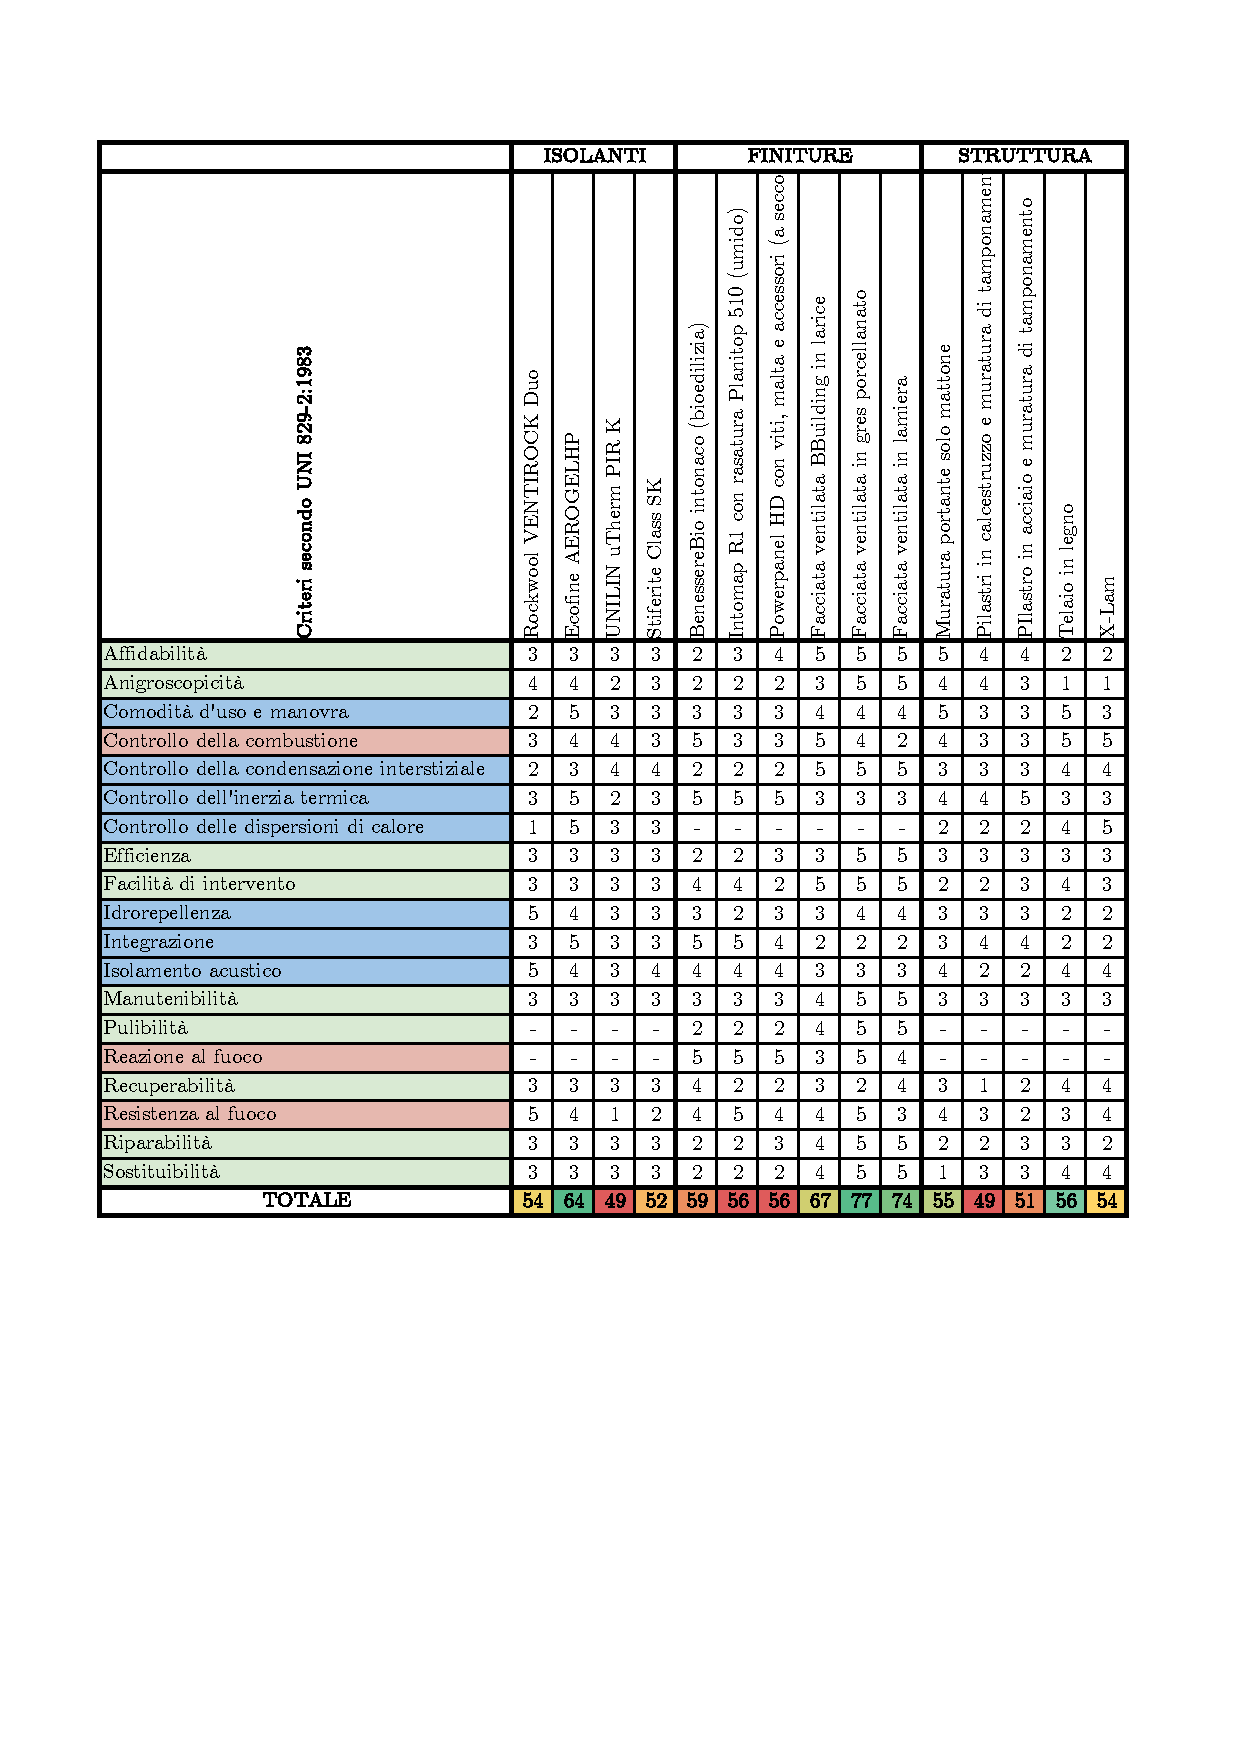
\includegraphics[width=0.9\textwidth]{img/AnalisiValore.pdf}
    \caption[Analisi del valore]{%
\scriptsize
\textbf{Affidabilità:} Capacità di mantenere sensibilmente invariata nel tempo la propria qualità in condizioni d'uso determinate
\textbf{Anigroscopicità:} Attitudine a non subire mutamenti di aspetto e/o morfologia, di dimensione e comportamento in seguito ad assorbimento di acqua o di vapor d'acqua
\textbf{Comodità d'uso e manovra:} Attitudine a presentare opportune caratteristiche di funzionalità, di facilità d'uso, di manovrabilità
\textbf{Controllo della combustione:} Realizzazione e mantenimento di condizioni tali da produrre processi di combustione a massimo rendimento di trasformazione e minima produzione di scorie e sostanze inquinanti
\textbf{Controllo della condensazione interstiziale:} Attitudine ad evitare la formazione di acqua di condensa all'interno degli elementi
\textbf{Controllo dell'inerzia termica:} Attitudine ad attenuare entro opportuni valori l'ampiezza di oscillazione della temperatura e a ritardarne di una opportuna entità l'effetto
\textbf{Controllo delle dispersioni di calore:} Contenimento entro determinati livelli delle perdite di calore per conduzione, convezione e irraggiamento
\textbf{Efficienza:} Capacità costante di rendimento nel funzionamento
\textbf{Facilità di intervento:} Possibilità di operare ispezioni, manutenzione e ripristini in modo agevole
\textbf{Idrorepellenza:} Attitudine a non essere penetrato da fluidi liquidi
\textbf{Integrazione:} Attitudine alla connessione funzionale e dimensionale
\textbf{Isolamento acustico:} Attitudine a fornire un'adeguata resistenza al passaggio di rumori
\textbf{Manutenibilità:} Possibilità di conformità a condizioni prestabilite entro un dato periodo di tempo in cui è compiuta l'azione di manutenzione
\textbf{Pulibilità:} Attitudine a consentire la rimozione di sporcizia e sostanze indesiderate
\textbf{Reazione al fuoco:} Grado di partecipazione di un materiale combustibile ad un fuoco al quale è sottoposto
\textbf{Recuperabilità:} Attitudine alla riutilizzazione di materiali o di elementi tecnici dopo demolizione o rimozione
\textbf{Resistenza al fuoco:} Attitudine a conservare, entro limiti determinati, per un intervallo di tempo determinato, le prestazioni fornite
\textbf{Riparabilità:} Attitudine a ripristinare l'integrità, la funzionalità e l'efficienza di parti o oggetti guasti 
\textbf{Sostituibilità:} Attitudine a consentire la collocazione di elementi tecnici al posto di altri}
\label{fig:AnalisiValore}
\end{figure}
        \section{Struttura}
Per quanto riguarda la struttura sono stati scelte diverse tipologie di soluzioni edilizie. 
Alcune di esse sono a muratura portante (caso coincidente con la soluzione zero di partenza) e altre presentano un telaio. 
Per queste ultime è stato calcolato anche la quota parte del tamponamento e non solo la parte strutturale. 
Un elenco è riportato nella tabella \ref{MaterialiStruttura}.
\begin{table}[htbp]
\caption{Elenco dei materiali strutturali presi in considerazione e descrizione sintetica delle loro caratteristiche.}
\label{MaterialiStruttura}
\centering
\begin{tabularx}{\textwidth}{rXX}
    \toprule
        \textbf{A} & \textbf{Muratura portante in laterizio} & Pannello rigido in lana di roccia non rivestito a doppia densità. 
        Adatto sia a isolamento termico che acustico, con ottimo comportamento al fuoco. 
        Ottima stabilità dimensionale e prestazionale. \\\midrule
        \textbf{B} & \textbf{Telaio in calcestruzzo e tamponamento in laterizio} & Struttura del telaio realizzata con pilastri in calcestruzzo armato classe XC0 di spessore $30\times\SI{30}{\centi\meter}$ e da travi di analoga tipologia con una dimensione $50\times\SI{30}{\centi\meter}$. Tamponamento realizzato con laterizi alveolati di spessore \SI{12}{\centi\meter}. \\\midrule
        \textbf{C} & \textbf{Telaio in acciaio e tamponamento in laterizio} & Struttura realizzata con pilastri HEA200 e travi IPE120, con muratura in tamponamento con tavolato in laterizio alveolato da \SI{12}{\centi\meter}\\\midrule
        \textbf{D} & \textbf{Telaio in legno con chiusura in fibrogesso} & Pareti a telaio in montanti e traversi di legno massello in abete. Le pareti sono costituite da montanti e traversi di sezione 12 per \SI{8}{\centi\meter} disposti ad interasse tra 55 e \SI{65}{\centi\meter}, giuntati con apposita ferramenta metallica, strutturalmente controventate nel loro piano con una doppia lastra in fibrogesso. \\\midrule
        \textbf{E} & \textbf{X-LAM} & Pannelli strutturali di legno multistrato X-LAM in legno di abete. Pannelli in 5 strati per uno spessore totale di \SI{10}{\centi\meter}. Ditta produttrice KLH.\\
    \bottomrule
\end{tabularx}
\end{table}
Nello scegliere gli spessori di queste soluzioni. si è cercato di dare una sensatezza strutturale ed un'uniformità generale.

Tra gli allegati disponibili a fine della relazione, in particolare a pagina \pageref{STRUTcostoMateriale}, è riportato il computo metrico estimativo relativo alla struttura, per il quale si è utilizzato esclusivamente i valori da prezzario.

Come criteri di paragone sono stati presi in considerazione, oltre al costo del materiale, anche il tempo di posa e lo spessore minore. 
Si è valutato come molto incidente soprattutto il primo, perché il tempo di costruzione può cambiare radicalmente tra una soluzione costruita in opera ed una prefabbricata.
Per questo motivo è stato elaborato il costo della manodopera, riportato nella tabella \ref{STRUTtempario} a pagina \pageref{STRUTtempario}. 
\begin{landscape}
\begin{table}[p]
\caption[Analisi costi della manodopera della parte strutturale esterna]{Analisi costi della manodopera della parte strutturale esterna. Dati presi dal tempario \cite{grosso2007tempario}. Per quanto riguarda la soluzione D il costo della manodopera è stato direttamente inserito in termini percentuali (il \SI{10}{\percent}) all'interno del costo totale finale. I dati dell'X-LAM della soluzione E sono stati ottenuti ri-elaborando dei computi metrici estimativi effettuati dall'azienda WoodCape SRL}
\label{STRUTtempario}
\centering\scriptsize
\begin{tabular}{llllrrrrrr}
\toprule
 &  Codice & Descrizione & u.m. & \multicolumn{1}{l}{Quant. ore} & \multicolumn{1}{l}{Quantità} & \multicolumn{1}{l}{Ore} & \multicolumn{1}{l}{Costo operaio} & \multicolumn{1}{l}{Totale (\teuro)} & \multicolumn{1}{l}{Costo totale}\\
  &   &  &  & \multicolumn{1}{l}{in cent. d'ora} & \multicolumn{1}{c}{(h)} & \multicolumn{1}{l}{} & \multicolumn{1}{l}{per ora (\teuro / h)} & \multicolumn{1}{l}{} & \multicolumn{1}{l}{manodopera (\teuro)}\\\midrule
\multirow{4}{*}{A} & TOC.130.330.f & Muratura monostrato in laterizio 30 cm & m2 & 0,6 & 198,24 & 118,94 & 30,99 & 3686,07 & \multirow{4}{*}{5.228,96} \\
 & TOC.100.110 & Conglomerato (cordolo) & m3 & 0,3 & 8,50 & 2,55 & 30,99 & 78,99 &  \\
 & TOC.100.300.c & Casseforme orizzontale cordolo & m2 & 0,48 & 84,96 & 40,78 & 30,99 & 1.263,80 &  \\
 & TOC.100.170.b & Armatura cordolo & kg & 0,019 & 339,84 & 6,46 & 30,99 & 200,10 &  \\\midrule
\multirow{5}{*}{B} & TOC.100.110 & Conglomerato (pilastri e travi) & m3 & 0,3 & 107,88 & 32,36 & 30,99 & 1.002,96 & \multirow{5}{*}{28.050,00} \\
 & TOC.100.220 & Casseforme pilastri & m2 & 0,48 & 369,60 & 177,41 & 30,99 & 5.497,87 &  \\
 & TOC.100.250 & Casseforme travi + sostegni & m2 & 0,96 & 293,92 & 282,16 & 30,99 & 8.744,24 &  \\
 & TOC.100.170.b & Armatura pilastri e travi & kg & 0,019 & 5.156,40 & 97,97 & 30,99 & 3.036,14 &  \\
 & TOC.130.330.c & Laterizi tamponamento 15 cm & m2 & 0,52 & 606,20 & 315,22 & 30,99 & 9.768,79 &  \\\midrule
\multirow{2}{*}{C} & TOC.160.110.b & pilastri e travi in acciaio & kg & 36,72 & 15.807,28 & 395,18 & 36,97 & 14.609,88 & 24.378,67 \\
 & TOC.130.330.c & Laterizi tamponamento 15 cm & m2 & 60,88 & 606,20 & 315,22 & 30,99 & 9.768,79 &  \\\midrule
D & \multicolumn{9}{c}{---} \\\midrule
E & Da azienda woodcape & Pareti strutturali perimetrali (15\teuro/m2) & m2 &  & 660,80 &  & 36,97 &  & 9.912,00\\\bottomrule
\end{tabular}
\end{table}
\end{landscape}
Alcuni dei materiali, data la loro natura, hanno permesso di utilizzare uno spessore ben minore, pertanto si è considerata anche la vendita della superficie risparmiata, con i parametri descritti al paragrafo precedente.

In tabella \ref{STRUTvincitore} viene riportato il resoconto dell'analisi sommando le quote parti del costo del materiale, costo manodopera e della superficie venduta.
\begin{table}[tb]
\caption[Analisi della struttura perimetrale]{Analisi della struttura perimetrale in cui si somma il costo del materiale, il costo di posa in opera e la superficie guadagnata (Sg) vendendo lo spazio disponibile grazie allo spessore minore secondi i parametri riportati all'inizio di questo capitolo. Con differenza relativa si intende il costo totale rapportato rispetto alla soluzione zero A.}
\label{STRUTvincitore}
\centering\scriptsize
\begin{tabular}{lrrrrrrr}
\toprule
\multicolumn{1}{c}{} & \multicolumn{1}{c}{Costo materiale} & \multicolumn{1}{c}{Costo tempario} & \multicolumn{1}{c}{Spessore} & \multicolumn{1}{c}{Sup. guad. (Sg)} & \multicolumn{1}{c}{Vendita Sg} &  \multicolumn{1}{c}{Costo Tot.} & \multicolumn{1}{c}{Diff. relativa} \\
\multicolumn{1}{c}{} & \multicolumn{1}{c}{\teuro} & \multicolumn{1}{c}{\teuro} & \multicolumn{1}{c}{m} & \multicolumn{1}{c}{mq} & \multicolumn{1}{c}{\teuro} &  \multicolumn{1}{c}{\teuro} & \multicolumn{1}{c}{\teuro} \\\midrule
A & 46.102 & 5.229 & 0,30 & 0,00 & 0,000 & \cellcolor[HTML]{DAD06E}51.331 & \cellcolor[HTML]{DAD06E}0,000 \\
B & 99.640 & 28.050 & 0,30 & 0,00 & 0,000 & \cellcolor[HTML]{E67C73}127.690 & \cellcolor[HTML]{E67C73}-76.359 \\
C & 92.857 & 24.379 & 0,20 & 9,44 & 28.320 & \cellcolor[HTML]{F3AB6C}88.916 & \cellcolor[HTML]{F3AB6C}-37.585 \\
D & 96.322 & 9.634 & 0,12 & 16,99 & 50.976 & \cellcolor[HTML]{FFD666}54.980 & \cellcolor[HTML]{FFD666}-3.649 \\
E & 84.969 & 9.912 & 0,10 & 18,88 & 56.640 & \cellcolor[HTML]{57BB8A}38.241 & \cellcolor[HTML]{57BB8A}13.089
\\\bottomrule
\end{tabular}
\end{table}
Se ne è evidenziata la differenza rispetto alla struttura zero, ottenendo come materiale economicamente più vantaggioso per la parete esterna l'\xlam.
Tale risultato è dato dall'esiguo spessore che si può utilizzare utilizzando una parete in \xlam{} e che nel caso nelle pareti esterne, riesce a recuperarne il costo ben maggiore del materiale.


        \section{Isolante}
Sono stati analizzati 4 isolanti con caratteristiche e soprattutto con costi molto differenti.
\begin{table}[H]
\caption{Elenco degli isolanti presi in considerazione e descrizione sintetica delle loro caratteristiche.}
\centering
\begin{tabularx}{\textwidth}{rXX}
    \toprule
        \textbf{A} & \textbf{Rockwool VENTIROCK Duo} & Pannello rigido in lana di roccia non rivestito a doppia densità. 
        Adatto sia a isolamento termico che acustico, con ottimo comportamento al fuoco. 
        Ottima stabilità dimensionale e prestazionale. \\\midrule
        \textbf{B} & \textbf{Ecofine AEROGELHP} & Pannello termoisolante in aerogel con matrice di supporto in fibra minerale, ininfiammabile, permeabile al vapore, senza rivestimento. 
        Ottimo comportamento al fuoco. 
        Indicato in generale in tutte le applicazioni in cui si desideri o si sia vincolati a contenere lo spessore.\\\midrule
        \textbf{C} & \textbf{UNILIN uTherm PIR K} & Panello isolante PIR ad alte prestazioni con un rivestimento multistrato di carta metallizzata su entrambi i lati. 
        Molto leggero e facile da posare.\\\midrule
        \textbf{D} & \textbf{Stiferite Class SK} & Pannello sandwich costituito da un componente isolante in schiuma polyiso, rivestito su entrambe le facce con velo vetro saturato.\\
    \bottomrule
\end{tabularx}
\end{table}
Per trovare l'isolante più conveniente è stato fissato come parametro la resistenza termica dell'isolante a spessore maggiore, ovvero l'isolante A spesso \SI{14}{\centi\metre}.
\[R_A = \frac{s}{\lambda}=\frac{\SI{0.14}{m}}{\SI{0.035}{W/mK}}=\SI{4}{m^2K\per W}\]
Con questo parametro sono stati trovati gli spessori degli altri isolanti che permettessero di equiparare (tenendo conto degli spessori commerciali) la resistenza. 
Ottenendo così i dati di tabella \ref{tab:Isolanti}.
\begin{table}[htb]
\centering
\caption[Confronto degli spessori degli isolanti a parità di resistenza termica]{Spessori isolanti a parità di resistenza termica voluta pari a \SI{4}{m^2K/W}. Il prezzo unitario si riferisce al costo del solo materiale, senza trasporti e installazione.}
\label{tab:Isolanti}
\begin{tabular}{@{}rrrr@{}}
\toprule
  & Conducibilità & Spessore & Prezzo unitario \\ 
  & W/mK          & m        & euro/mq            \\ \midrule
A & 0,035         & 0,14     & 19,00           \\
B & 0,015         & 0,06     & 362,00          \\
C & 0,022         & 0,10     & 51,00           \\
D & 0,025         & 0,10     & 29,00           \\ \bottomrule
\end{tabular}%
\end{table}

Per decretare quale avesse il costo maggiore è stata presa in considerazione la superficie risparmiata grazie allo spessore minore degli isolanti B, C, D.
\e stato analizzato sia la vendita con un  prezzo di vendita di \SI{3000}{\teuro / \square\metre}, che di affitto di \SI{10.41}{\teuro /\square\metre mese }. Valori che sono stati presi analizzando i prezzi di mercato forniti dall'Agenzia delle Entrate a Trento.
\begin{table}[htb]
\caption[Analisi dell'isolante]{Analisi considerando il costo del materiale e il guadagno vendendo o affittando la superficie guadagnata grazie allo spessore ridotto di quell'isolante rispetto alla soluzione peggiore A. 
Dove con ogni riga si intende 1, 2, o 10 piani.
Evidenziati sono i guadagni o le perdite nel caso di vendita e utlizzando una superficie di due piani.}
\label{ISOvincitore}
\centering\scriptsize
\begin{tabular}{@{}crrrrrrrr@{}}
\toprule
& \multicolumn{1}{c}{Cost.Mat.} & \multicolumn{1}{c}{Diff. A} & \multicolumn{1}{c}{Sup. risp.} & \multicolumn{1}{c}{Vendita} &\multicolumn{1}{c}{Aff. 1} & \multicolumn{1}{c}{Aff. 10} & \multicolumn{1}{c}{Guad. Ven.} & \multicolumn{1}{c}{Guad. Aff.}  \\ 
& \multicolumn{1}{c}{\teuro} & \multicolumn{1}{c}{\teuro} & \multicolumn{1}{c}{\SI{}{\square\metre}} & \multicolumn{1}{c}{\teuro} &\multicolumn{1}{c}{\teuro} & \multicolumn{1}{c}{\teuro} & \multicolumn{1}{c}{\teuro} & \multicolumn{1}{c}{\teuro}  \\ \midrule
\multirow{3}{*}{A}   & 6.277,60                                                     & \multicolumn{1}{c}{/}                                & \multicolumn{1}{c}{/}          & \multicolumn{1}{c}{/}               & \multicolumn{1}{c}{/}               & \multicolumn{1}{c}{/}                                      & \multicolumn{1}{c}{/}                                              & \multicolumn{1}{c}{/} \\
                     & 12.555,20                                                    & \multicolumn{1}{c}{/}                                & \multicolumn{1}{c}{/}          & \multicolumn{1}{c}{/}               & \multicolumn{1}{c}{/}               & \multicolumn{1}{c}{/}                                      & \multicolumn{1}{c}{/}                                              & \multicolumn{1}{c}{/} \\
                     & 62.776,00                                                    & \multicolumn{1}{c}{/}                                & \multicolumn{1}{c}{/}          & \multicolumn{1}{c}{/}               & \multicolumn{1}{c}{/}               & \multicolumn{1}{c}{/}                                      & \multicolumn{1}{c}{/}                                              & \multicolumn{1}{c}{/} \\\midrule
\multirow{3}{*}{B}   & 119.604,80                                                   & 113.327,20                                           & 7,58                           & 22.740,00                           & 946,89                              & 9.468,94                                                   & -90.587,20                                                         & -103.858,26           \\
                     & 239.209,60                                                   & 226.654,40                                           & 15,17                          & 45.510,00                           & 1.895,04                            & 18.950,36                                                  & \cellcolor[HTML]{FD6864}-181.144,40                                                        & -207.704,04           \\
                     & 1.196.048,00                                                 & 1.133.272,00                                         & 75,84                          & 227.520,00                          & 9.473,93                            & 94.739,33                                                  & -905.752,00                                                        & -1.038.532,67         \\\midrule
\multirow{3}{*}{C}   & 16.850,40                                                    & 10.572,80                                            & 3,79                           & 11.370,00                           & 473,45                              & 4.734,47                                                   & 797,20                                                             & -5.838,33             \\
                     & 33.700,80                                                    & 21.145,60                                            & 7,58                           & 22.740,00                           & 946,89                              & 9.468,94                                                   & \cellcolor[HTML]{FFFC9E}1.594,40                                                           & -11.676,66            \\
                     & 168.504,00                                                   & 105.728,00                                           & 37,92                          & 113.760,00                          & 4.736,97                            & 47.369,66                                                  & 8.032,00                                                           & -58.358,34            \\\midrule
\multirow{3}{*}{D}   & 9.581,60                                                     & 3.304,00                                             & 3,79                           & 11.370,00                           & 473,45                              & 4.734,47                                                   & 8.066,00                                                           & 1.430,47              \\
                     & 19.163,20                                                    & 6.608,00                                             & 7,58                           & 22.740,00                           & 946,89                              & 9.468,94                                                   & \cellcolor[HTML]{67FD9A}16.132,00                                                          & 2.860,94              \\
                     & 95.816,00                                                    & 33.040,00                                            & 37,92                          & 113.760,00                          & 4.736,97                            & 47.369,66                                                  & 80.720,00                                                          & 14.329,66             \\ \bottomrule 
\end{tabular}
\end{table}

Nella tabella \ref{ISOvincitore} si sono riportati i confronti dei quattro isolanti riportando i valori rispetto all'isolante peggiore.
Valori che portano a dire che l'isolante vincitore è il quarto e permette di risparmiare \SI{16132.00}{\teuro} nel caso delle cinque villette a schiere di due piani.
Sono stati riportati -- per pura speculazione -- anche i dati relativi ad una possibile abitazione di 10 piani.
\e evidente il maggior risparmio con la soluzione D.

Nel confronto non sono stati tenuti in considerazione né il trasporto né il possibile guadagno dovuto al minor spazio occupato in cantiere dall'isolante.
Si è supposto infatti che l'origine delle fabbriche delle aziende produttrici fosse in una posizione tale da non variare significativamente il costo del trasporto. 
\e anche vero che l'isolante B -- quello con le maggiori prestazioni -- potrebbe richiedere un viaggio in meno, ma l'enorme differenza di costo intrinseco del materiale fa sì che ciò non incida.

Non sono stati presi in considerazione neanche la manutenzione né la tempistica di posa in opera, in quanto si è supposto fosse uguale per tutte le tipologie.
%%%

        \section{Rivestimento esterno}
\begin{table}[htbp]
\caption[Elenco dei rivestimenti esterni presi in considerazione e descrizione sintetica delle loro caratteristiche]{Elenco dei rivestimenti esterni presi in considerazione e descrizione sintetica delle loro caratteristiche. Per quelli con un asterisco $^\star$ è stata effettuata un'analisi dei prezzi.}
\label{MaterialiRIV}
\centering
\begin{tabularx}{\textwidth}{rXX}
    \toprule
        \textbf{A} & \textbf{BenessereBio intonaco $\,^\star$} & Biointonaco termo-deumidificante, antimuffa e anti condensa. 
        Adatto a tutti i tipi di muro. Traspirante ed ad alta efficienza energetica. \\\midrule
        \textbf{B} & \textbf{Intomap R1 $\,^\star$} & Intonaco di fondo su murature miste, laterizio nuovo, blocchi in calcestruzzo e cemento armato gettato.  Buona adesione, particolarmente indicato per essere applicato con intonacatrice. 
        Rasatura con Planitop 510 in calce-cemento a tessitura fine.\\\midrule
        \textbf{C} & \textbf{Powerpanel HD $\,^\star$} & Rivestimento per ambienti esterni con lastre in conglomerato cementizio, di peso ridotto, facili da lavorare e durevoli agli agenti atmosferici.\\\midrule
        \textbf{D} & \textbf{Facciata ventilata BBuilding in larice} & Costituita da pannelli premontati in stabilimento composti da una sottostruttura portante e da doghe posate orizzontalmente, completamente realizzata in legno di larice massello non impregnato.\\\midrule
        \textbf{E} & \textbf{Facciata ventilata gres porcellanato} & Sistema strutturale di rivestimento esterno degli edifici per combinare estetica, funzionalità, manutenzione ed efficienza energetica. \\\midrule
        \textbf{F} & \textbf{Facciata ventilata in lamiera Prefa} & Possono essere utilizzate sia per esterni che per interni per rivestire pareti e soffitti. Il fissaggio a scomparsa mediante un sistema ad incastro maschio - femmina garantisce un'estetica gradevole. Si ottengono facciate di facile manutenzione e all'avanguardia per molti decenni.\\
    \bottomrule
\end{tabularx}
\end{table}
\begin{landscape}
\begin{table}[p]
\caption{Piano di manutenzione del rivestimento esterno. 
\e stato considerato rispetto i 30 anni di vita utile del migliore, ovvero la facciata ventilata in lamiera Prefa.}
\label{RIV_PianoManutenzione}
\centering\scriptsize
\begin{tabular}{@{}lllllrcr@{}}
\toprule
Elem. Tecnico & Tipologia Elem. & Tipologia & Soggeto & Cadenza & Costo singolo & Ripetizioni & \multicolumn{1}{l}{Costo} \\ 
Manutenibile & Tecnico & intervento & Esecutore & (Anni) & intervento (\teuro) & \multicolumn{1}{l}{previste} & \multicolumn{1}{c}{totale (\teuro)} \\ \midrule
\multirow{4}{*}{Intonaco} & \multirow{4}{*}{BenessereBio intonaco} & Controllo generale delle parti a vista & Utente & 0,5 &   0,00 & 60 &   0,00 \\
 &  & Pulizia delle superfici & Pittore & 10 &   6.608,00 & 2 &   13.216,00 \\
 &  & Sostituzione delle parti più soggette ad usura & Muratore & 10 &   891,09 & 2 &   1.782,18 \\
 &  &  &  &  &  & TOT &   14.998,18 \\ \midrule
\multirow{4}{*}{Intonaco} & \multirow{4}{*}{Intomap R1} & Controllo generale delle parti a vista & Utente & 0,5 &   0,00 & 60 &   0,00 \\
 &  & Pulizia delle superfici & Pittore & 10 &   6.608,00 & 2 &   13.216,00 \\
 &  & Sostituzione delle parti più soggette ad usura & Muratore & 10 &   995,83 & 2 &   1.991,65 \\
 &  &  &  &  &  & TOT &   15.207,65 \\ \midrule
\multirow{4}{*}{Rivestimento lapideo} & \multirow{4}{*}{Powerpanel HD} & Controllo generale delle parti a vista & Utente & 1 &   0,00 & 30 &   0,00 \\
 &  & Pulizia delle superfici con idropulitrice & Pittore & 10 &   5.286,40 & 2 &   10.572,80 \\
 &  & Sostituzione delle parti più soggette ad usura & Pavimentista & 10 &   1.984,05 & 2 &   3.968,10 \\
 &  &  &  &  &  & TOT &   14.540,90 \\\midrule
\multirow{4}{*}{Rivestimento ligneo} & \multirow{4}{*}{Facciata ventilata BBuilding} & Controllo generale delle parti a vista & Utente & 0,5 &   0,00 & 60 &   0,00 \\
 &  & Ripristino degli strati protettivi & Pittore & 10 &   7.486,86 & 2 &   14.973,73 \\
 &  & Sostituzione delle parti più soggette ad usura & Pavimentista & 10 &   5.088,16 & 2 &   10.176,32 \\
 &  &  &  &  &  & TOT &   25.150,05 \\ \midrule
\multirow{4}{*}{Rivestimento lapideo} & \multirow{4}{*}{Facciata ventilata gres} & Controllo generale delle parti a vista & Utente & 0,5 &   0,00 & 60 &   0,00 \\
 &  & Ripristino degli strati protettivi & Pittore & 10 &   2.808,40 & 2 &   5.616,80 \\
 &  & Sostituzione delle parti più soggette ad usura & Pavimentista & 10 &   2.940,56 & 2 &   5.881,12 \\
 &  &  &  &  &  & TOT &   11.497,92 \\\midrule
\multirow{2}{*}{Rivestimento metallico} & \multirow{2}{*}{Facciata ventilata lamiera} & Controllo generale delleparti a vista & Utente & 0,5 &   0,00 & 60 &   0,00 \\
 &  &  &  &  &  & TOT &   0,00 \\ \bottomrule
\end{tabular}
\end{table}
\end{landscape}
Per quanto riguarda il rivestimento esterno, non per tutti è stato possibile trovare direttamente il prezzo unitario nel prezzario. 
Pertanto, per quelli che in tabella \ref{MaterialiRIV} riportano un asterisco, è stato necessario eseguire un'analisi dei prezzi utilizzando i dati dichiarati dai produttori. 
Questo a causa della particolare natura di quel materiale e specifico di un'azienda in particolare, o relativamente nuovo sul mercato da esser aggiunto al prezzario della Provincia di Trento.

Nel caso del rivestimento esterno è stata valutata come molto incidente la manutenzione da attuare in corso d'opera, essendo il rivestimento esposto alle intemperie e non protetto come gli altri strati. 
Non è stato preso in considerazione il tempo di posa, perché si è supposto fosse simile tra tutti.
Nemmeno il parametro dello spessore è stato considerato, perché in questo caso sono tutti ben che minimo uguali.

A causa quindi della durata del materiale è stato creato un piano manutenzione esposto nella tabella \ref{RIV_PianoManutenzione} a pagina \pageref{RIV_PianoManutenzione}.

Nella tabella \ref{RIVvincitore} è riportato il sommario tra prezzi unitari finali e la manutenzione. 
Sono riportati infine i costi finali del rivestimento, evidenziando come la soluzione con l'intonaco A sia quella più conveniente in termini di costi totali.
\begin{table}[htb]
\caption[Analisi del rivestimento esterno]{Analisi del rivestimento esterno. Somma tra i costi del materiale e i costi di manutenzione. L'ultima colonna evidenza il minor costo finale della soluzione A.}
\label{RIVvincitore}
\centering\scriptsize
\begin{tabular}{@{}rrrrr@{}}
\toprule
& \multicolumn{1}{c}{Prezzo unitario} & \multicolumn{1}{c}{Costo materiale} & \multicolumn{1}{c}{Manutenzione} & \multicolumn{1}{c}{Costo}  \\ 
 & \multicolumn{1}{c}{\teuro/mq} & \multicolumn{1}{c}{\teuro} & \multicolumn{1}{c}{\teuro} & \multicolumn{1}{c}{\teuro} \\\midrule
A & 14,97 &  9.893,09 &  14.998,18 &  \cellcolor[HTML]{3FE52C}24.891,27 \\
B & 18,14 &  11.986,91 &  15.207,65 &  \cellcolor[HTML]{13AE14}27.194,56 \\
C & 46,05 &  30.429,84 &  14.540,90 &  \cellcolor[HTML]{CFE703}44.970,74 \\
D & 140,00 &  92.512,00 &  25.150,05 &  \cellcolor[HTML]{F66E51}117.662,05 \\
E & 75,00 &  49.560,00 &  11.497,92 &  \cellcolor[HTML]{FBDA59}61.057,92 \\
F & 130,00 &  85.904,00 &  0,00 &  \cellcolor[HTML]{FB813F}85.904,00 \\ \bottomrule
\end{tabular}
\end{table}

        %\section{Considerazioni sul vincitore}
%init
%Capitoli analisi intero edificio
    \chapter{Analisi di pareti interne e solai}
%Capitoli considerazioni sui vincitore e conclusioni
    \chapter{Considerazioni sui finalisti}
Si vuole ora analizzare più del dettaglio il confronto tra la soluzione zero in muratura portante e la struttura in X-LAM. 
Si è visto come l'X-LAM sia più vantaggioso nel caso si analizzano solamente le pareti esterne, perché grazie al suo spessore minore (a parità di prestazioni) permette di risparmiare molta superficie e quindi di rivenderla.
Questo però non è sufficiente a colmare il maggior costo intrinseco del materiale non appena si prende in considerazione l'intera struttura dell'edificio. 
Nei solai infatti, non c'è nessun guadagno dall'avere uno spessore minore, se non quello di avere un pacchetto meno spesso, ma ciò non si traduce in ricavi.

Si elencheranno ora delle opzioni per poter capire se abbia senso o meno, a fronte dei \SI{180000}{\teuro} in più, scegliere comunque la soluzione in X-LAM. 
O se invece è preferibile optare per la muratura portante perché i benefici non sono abbastanza.
\begin{quoting}
    CLT is cost-competitive because it already has thermal insulation, \omissis{} and for sure it might be a little bit more expensive in the beginning, but when you also include the maintenance costs it turns out be absulutely cost-competitive. - \textcite{mallo_outlook_2014}
\end{quoting}    
\paragraph{Tempi di costruzione}
Si è visto nel paragrafo dedicato alle strutture esterne, come il tempo sia stato molto incidente nel definire gli importi delle varie soluzioni adottate.
Non si è ancora considerato il cantiere nel suo intero insieme, considerando i tempi di attesa e di gestione.

Utilizzare un materiale che necessita di posa in opera, o uno che invece ha la sola necessità di essere assemblato, cambia radicalmente i tempi del cantiere.
Sebbene con l'X-LAM serva una gru per la posa dei pannelli, la posa e l'indurimento dei componenti in calcestruzzo del solaio in latero-cemento comporta un tempo che è dell'ordine di 1 o 2 mesi contro le 2-3 settimane necessarie con l'X-LAM. 
Avere un tempo di costruzione di alcune settimane in meno comporta sia la vendita anticipata: cosa che in alcune situazioni può significare enormi guadagni per il committente, che può iniziare ad avere un ritorno economico del proprio investimento in tempi molto più rapidi.
Sia costi di gestione del cantiere e di facilità di verifica della corretta posa enormemente minori. Avendo elementi prefabbricati realizzati tramite apposite macchine a taglio numerico CNC, tutti gli elementi hanno una perfetta dimensione rispetto il progetto. Non si avranno quindi possibilità di richiesta di varianti in corso d'opera dovute ad elementi che non si incastrano a causa di qualche centimetro diverso.

Per grandi strutture è differente anche il numero di operai che servono a realizzare la struttura. Utilizzando una struttura in X-LAM sono sufficienti tre persone per una normale unità familiare. Per ottenere lo stesso quantitativo di tempo utilizzando la muratura portante, sono necessarie almeno il doppio degli operai. Avendo così più costi di manodopera e più personale da riuscire a gestire all'interno del cantiere. 

Per riportare un esempio: il palazzo progettato da Land Lease a Meolbourne, ovvero il primo edificio di dieci piani ad essere costruito in X-LAM, è stato realizzato in appena 38 giorni. Comparandolo con un edificio simile costruito con telaio in calcestruzzo o con muratura portante, il tempo sale a 20 settimane \cite[39]{10storey}. 


\paragraph{X-LAM come isolante}
Nell'analisi del pacchetto isolante non si è considerato il fatto che l'X-LAM è ben più isolante rispetto la muratura portante. I due, infatti, hanno rispettivamente una conducibilità termica $\lambda$ di \SI{0.12}{} e di \SI{0.30}{W\per\metre K}.
Ciò consente di supporre che l'X-LAM potrebbe essere considerato come contribuente alla resistenza termica di parete. 

Mantenendo una resistenza voluta di \SI{4}{\square\metre K\per W} è possibile utilizzare \SI{2}{\centi\metre} in meno di isolante e ciò comporta due cose: si risparmiano altri due centimetri lungo tutto il perimetro, potendo ricavarne dalla vendita; si ha uno spessore isolante (utilizzando il vincitore D) ridotto a \SI{8}{\centi\metre} e che ha un prezzo unitario di \SI{23.73}{\teuro} al posto dei \SI{29.00}{\teuro} iniziali.

Questo si traduce in \SI{11370}{\teuro} recuperati dalla vendita e da \SI{3482.65}{\teuro} utilizzando l'isolante meno spesso.

Non solo. Se si considera l'intero \textit{Life Cycle Analysis} (LCA) avere molto isolante può comportare danni ambientali e di salubrità dell'ambiente interno \cite{reijnders_comprehensiveness_1999}. Avere un materiale che può in parte sostituirlo, sicuramente può aiutare. 
\paragraph{X-LAM come legno}
Utilizzare un prodotto eco-sostenibile come il legno comporta innumerevoli vantaggi dal punto di vista della salute \cite{EnergyCost}. 
Non solo: in termini economici si possono ottenere finanziamenti o mutui per la costruzione con determinati materiali. 

Utilizzando prodotti lignei è inoltre possibile acquisire vari punti extra nelle certificazioni energetiche quali Casa Clima o LEED. 
Certificazioni che potrebbero far aumentare non poco il valore immobiliare degli edifici costruiti. 

Un altro aspetto a vantaggio può essere l'opportunità di recuperare dei punti CAM a discapito di altri, in punti in cui magari, per certe situazioni, era impossibile da rispettare.

\textcite{mallo_outlook_2014}
\textcite{wcms_wood_nodate}
    %ALLEGATI IN FONDO A TUTTO:
\appendix
\renewcommand{\thechapter}{Allegati} %Toglie A,B,C delle appendici del TOC sostituendolo con "Allegati"
%Funziona solo perché c'è solo un appendice sennò non avrebbe senso
\titleformat{\chapter}%toglie A, B, C e sposta il nome a sinistra
        {\normalfont\Huge\bfseries}{}{0em}{} 
\chapter[]{Allegati} %Nell'indice non ha nome []
\begin{enumerate}
    \item Piante edificio
    \item Zonizzazione dello stato zero
    \item WBS stato zero
    \item Computo metrico estimativo struttura perimetrale
    \item Computo metrico estimativo struttura pareti interne e solai intermedi e di copertura
\end{enumerate}
%Piante edificio:
%I pdf originali sono in A3 a scala 1:50 in realtà. Ora è diventato in 1:100 A4
\label{piante}
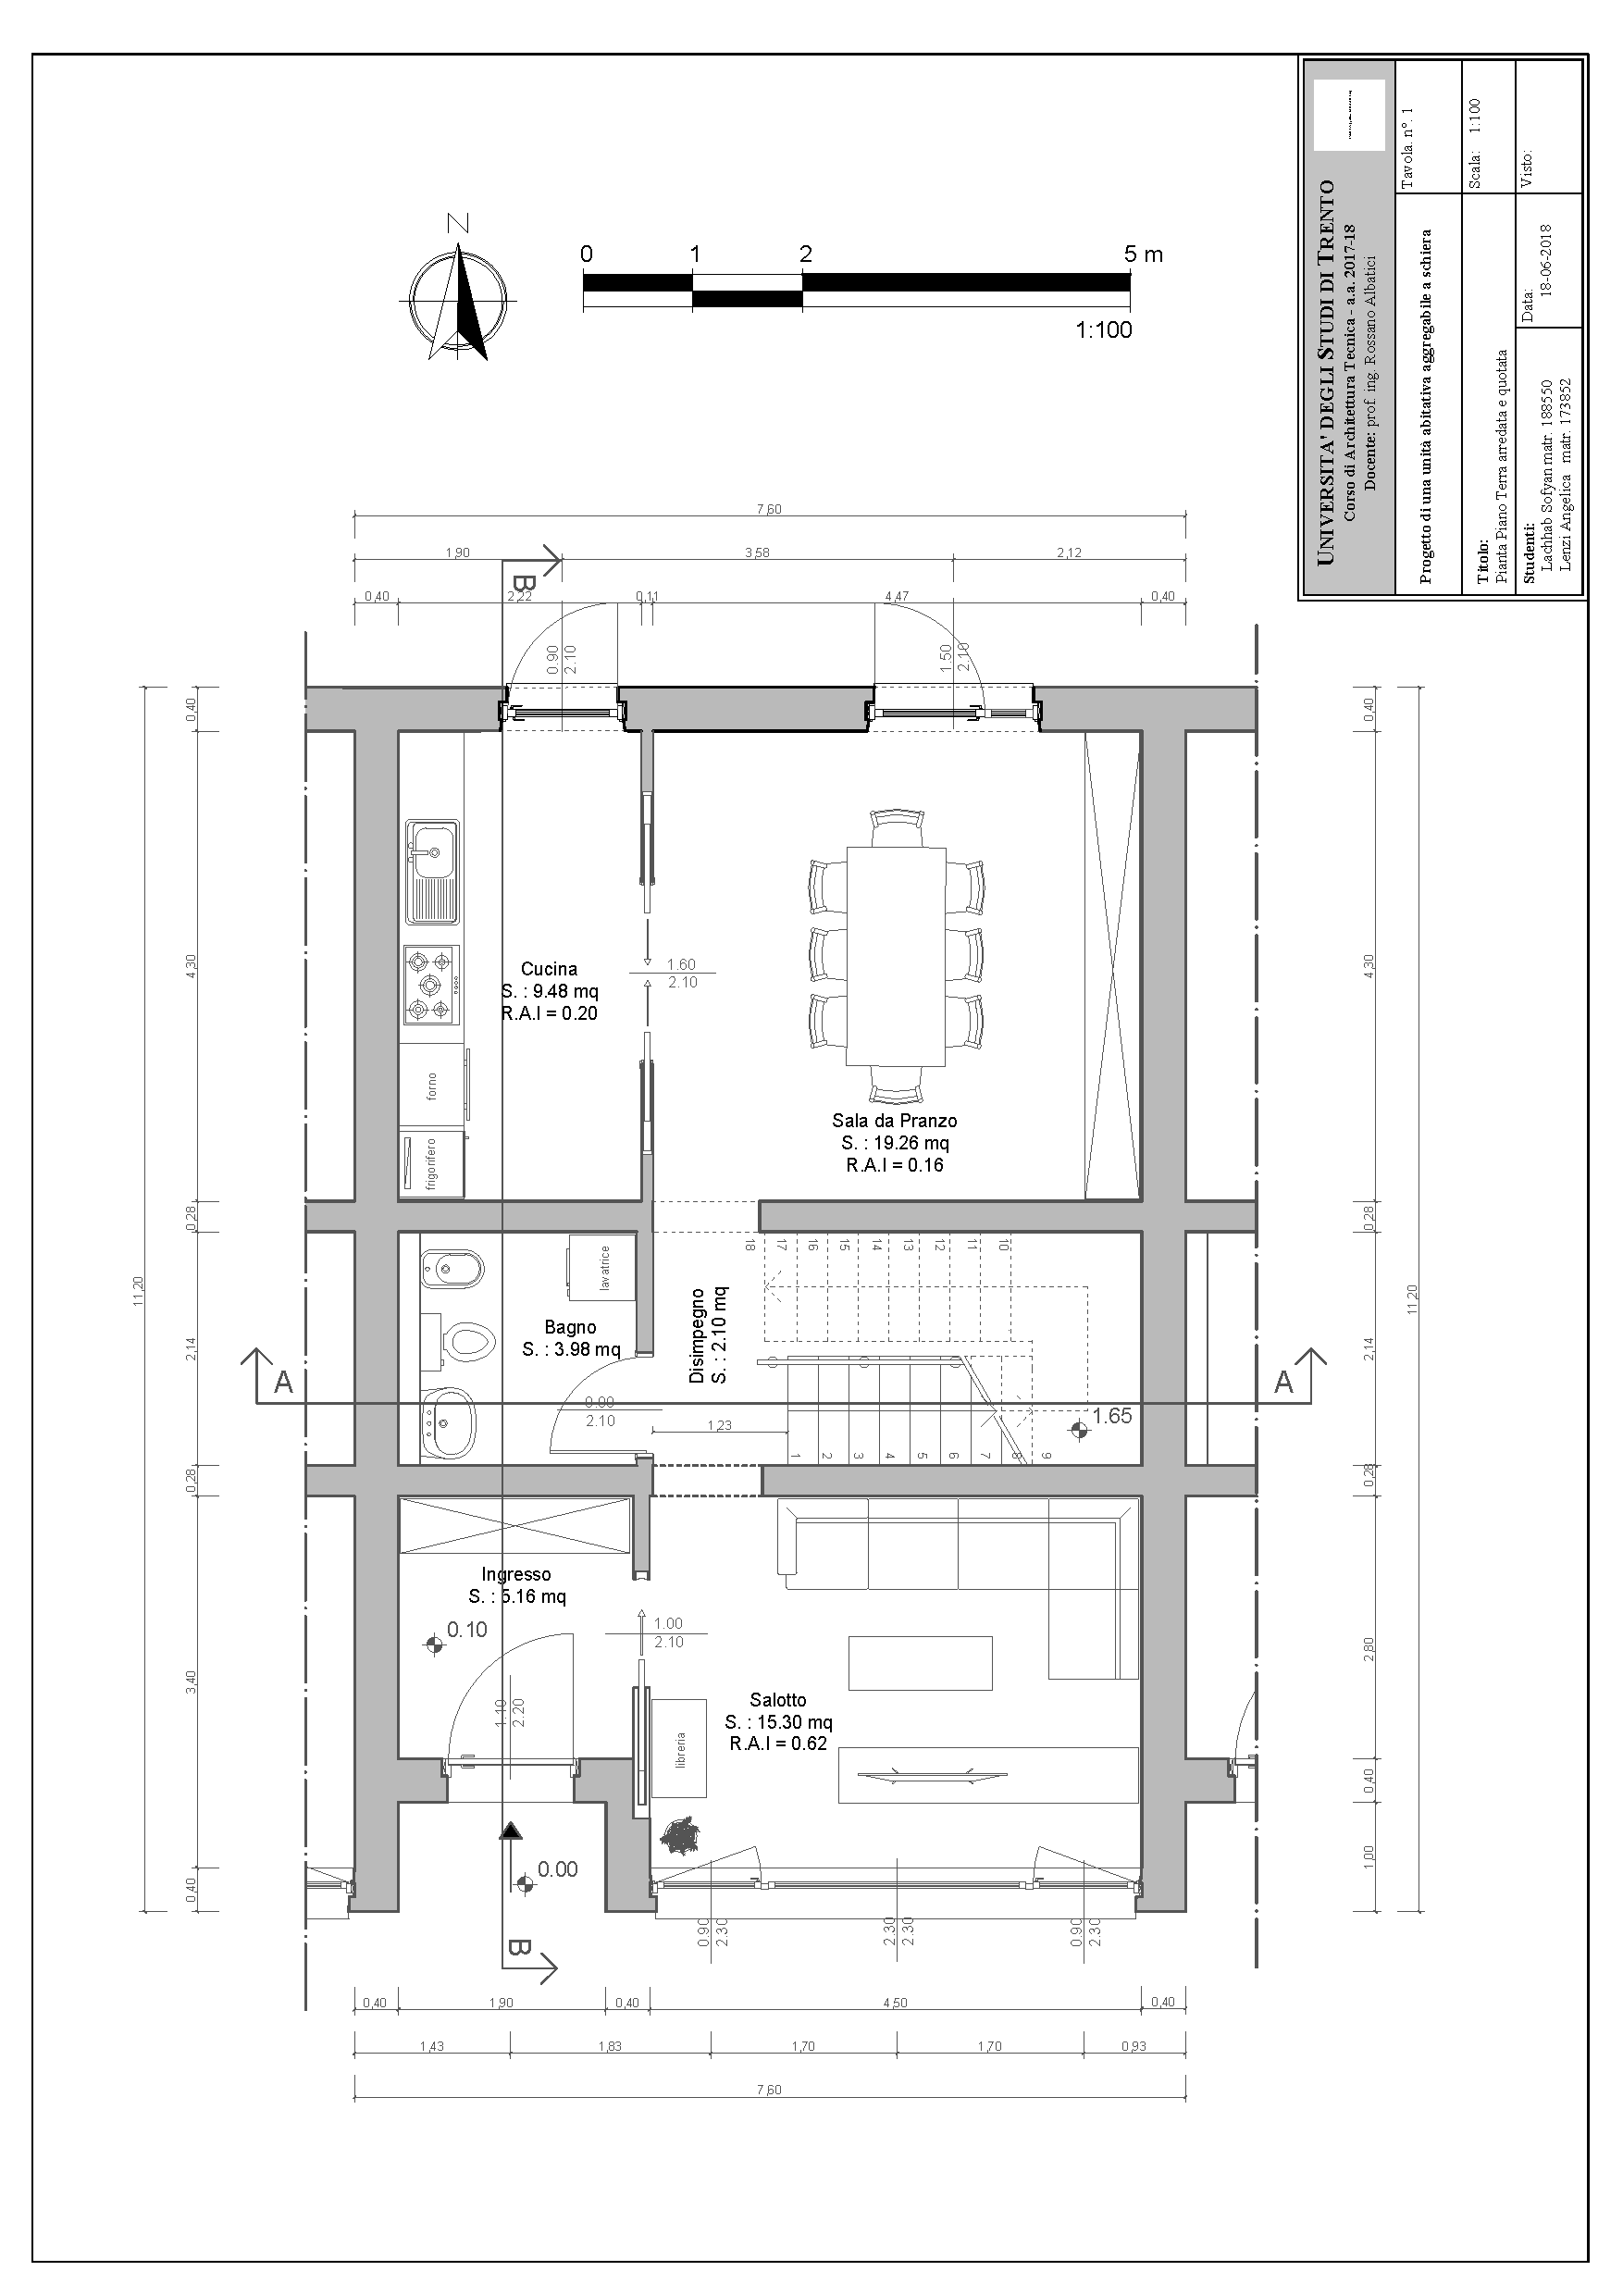
\includepdf[pages={1},pagecommand={\thispagestyle{plain}}]{img/PiantaTerraA3scala50.pdf}
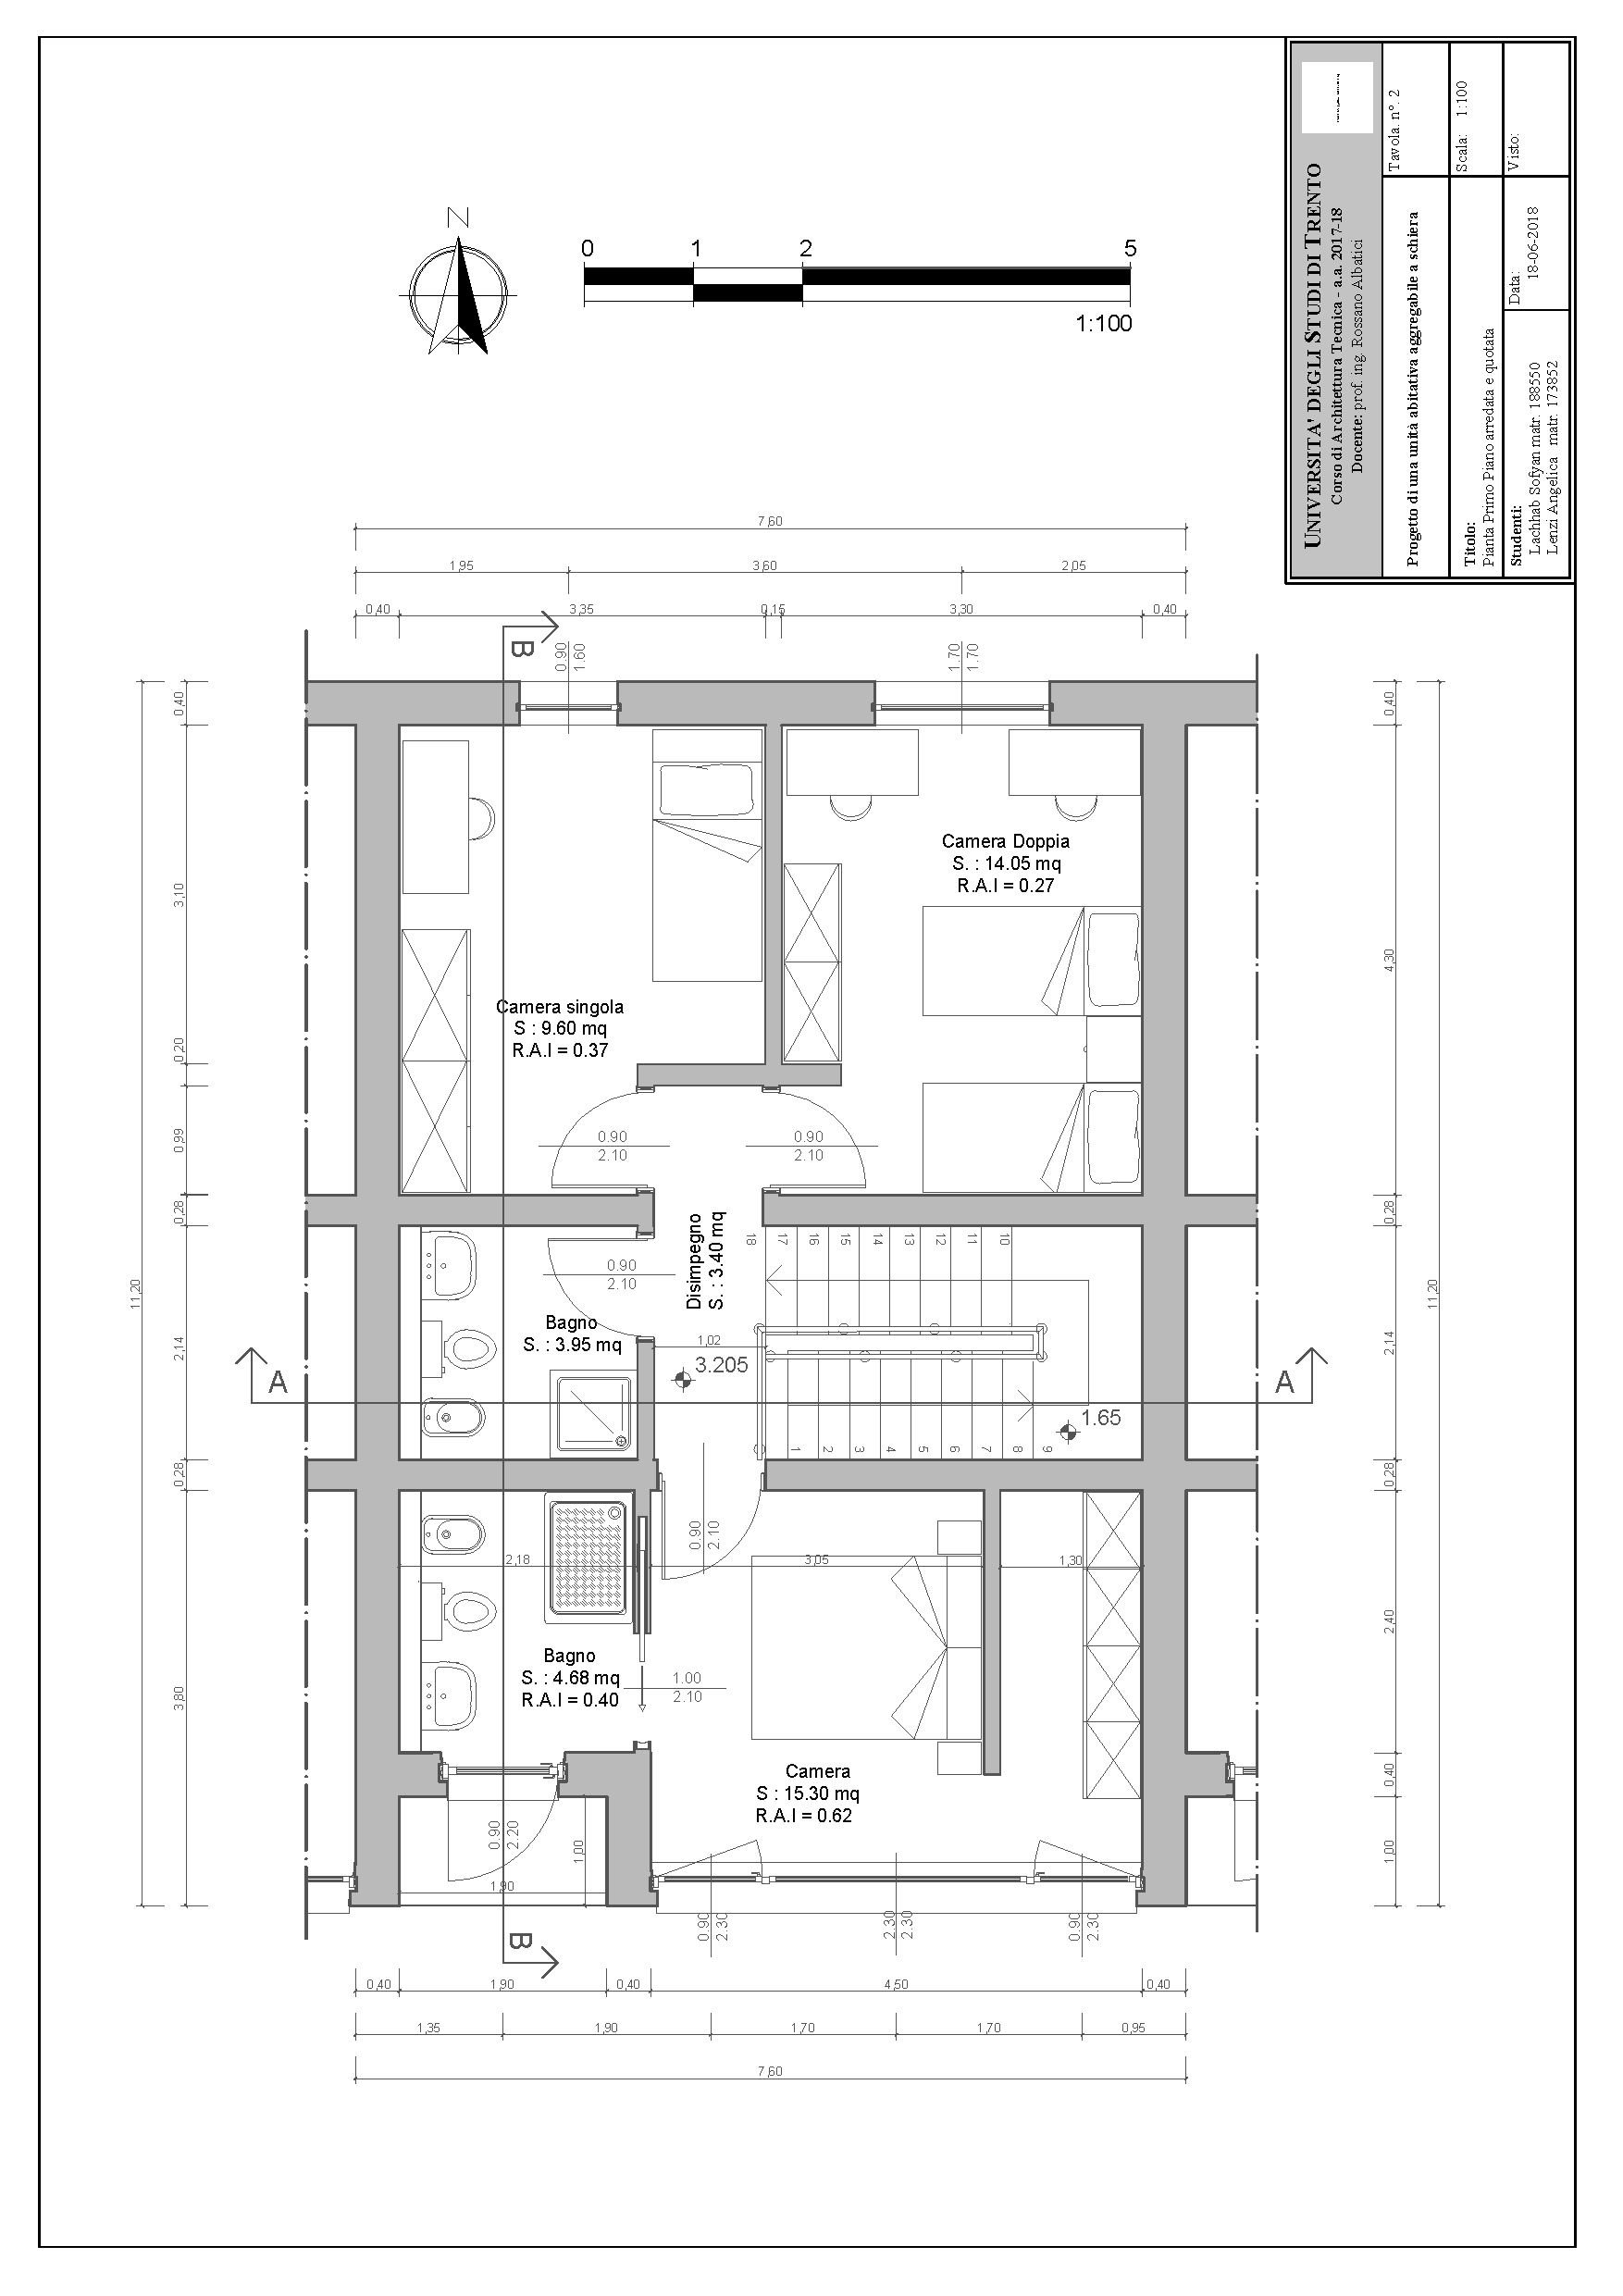
\includepdf[pages={1},pagecommand={\thispagestyle{plain}}]{img/PiantaPrimoA3scala50.pdf}
%Zona ubicazione edificio
\label{Edificio}
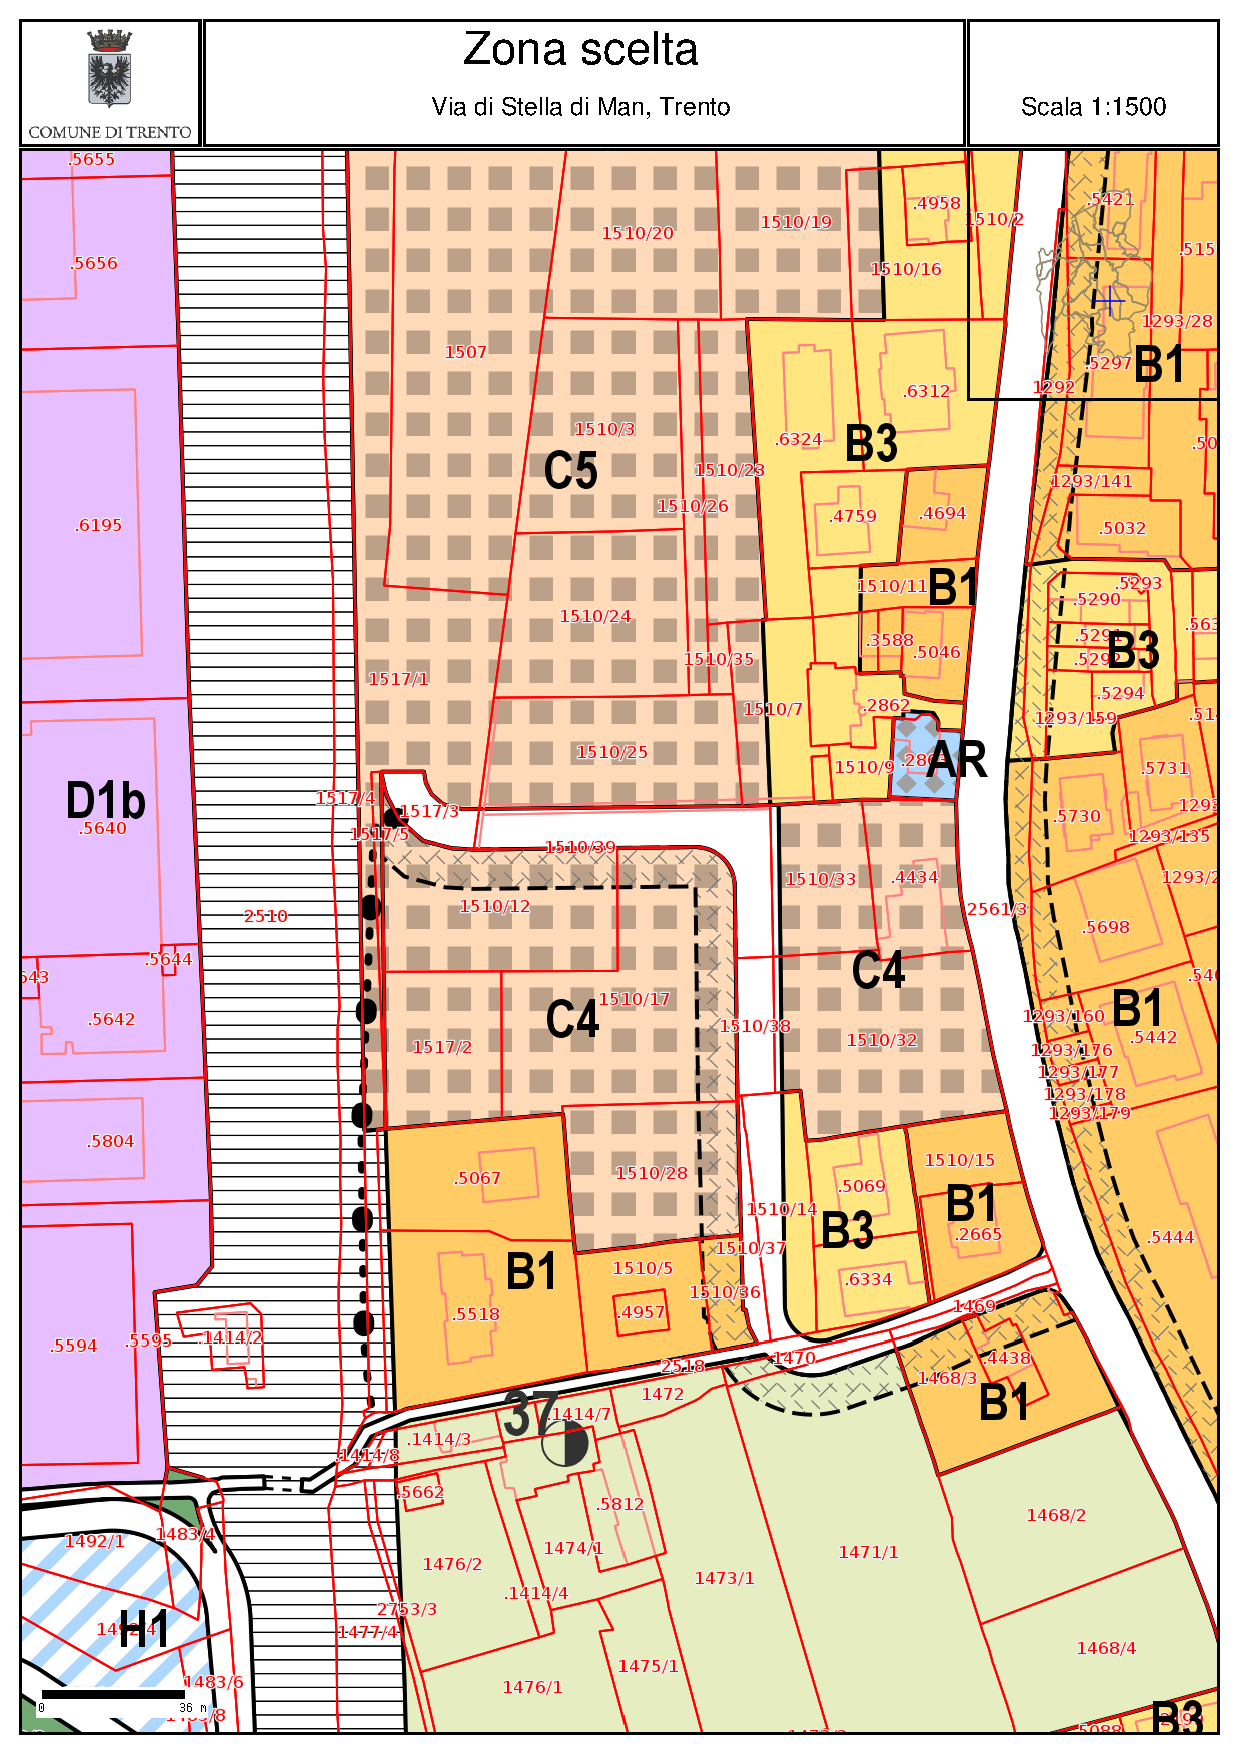
\includepdf[pages={1,2},pagecommand={\thispagestyle{plain}}]{img/Zonizzazione1.pdf}
\includepdf[pages={1},pagecommand={\thispagestyle{plain}}]{img/Zonizzazione2.pdf}
%WBS:
\label{WBS}
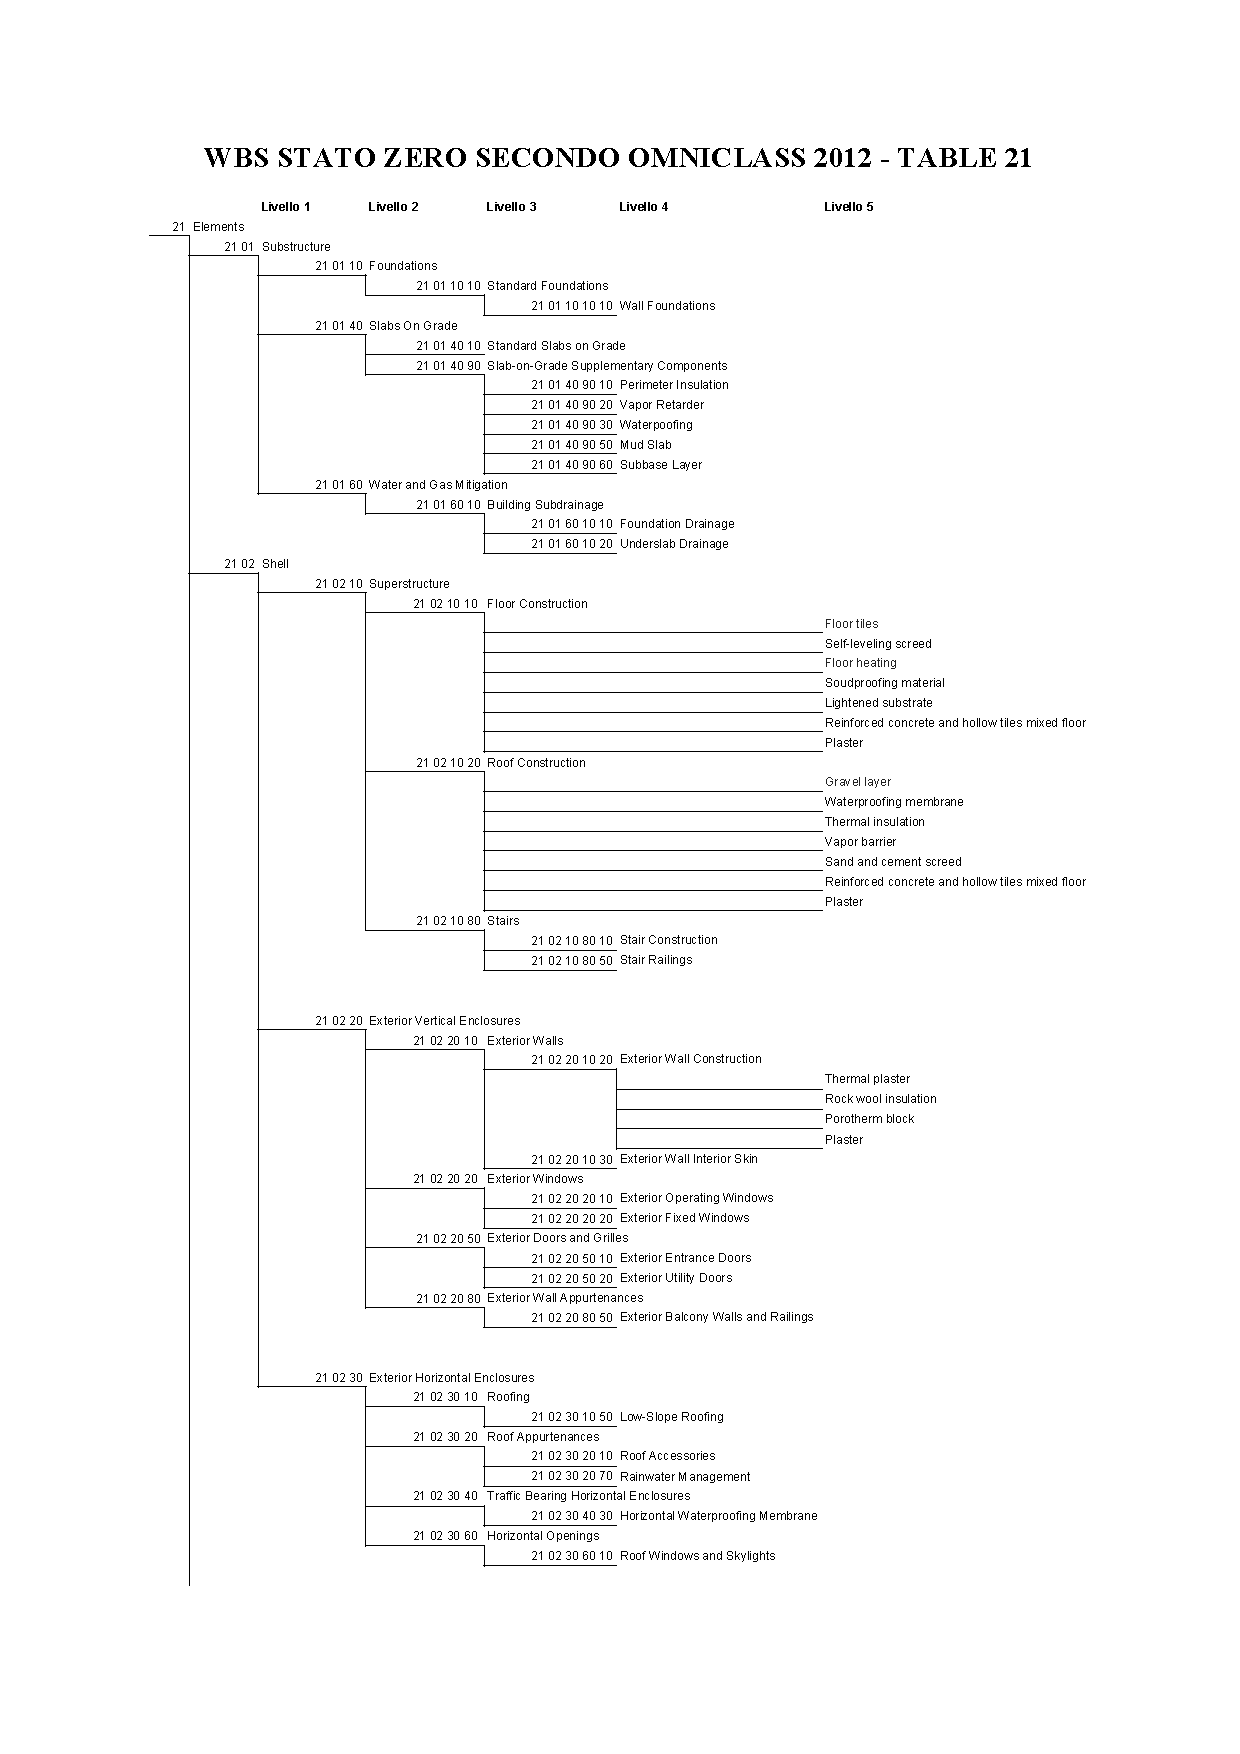
\includepdf[pages={1,2},pagecommand={\thispagestyle{plain}}]{img/WBStable21.pdf}
%Conputo strutture perimetrali:
\label{STRUTcostoMateriale}
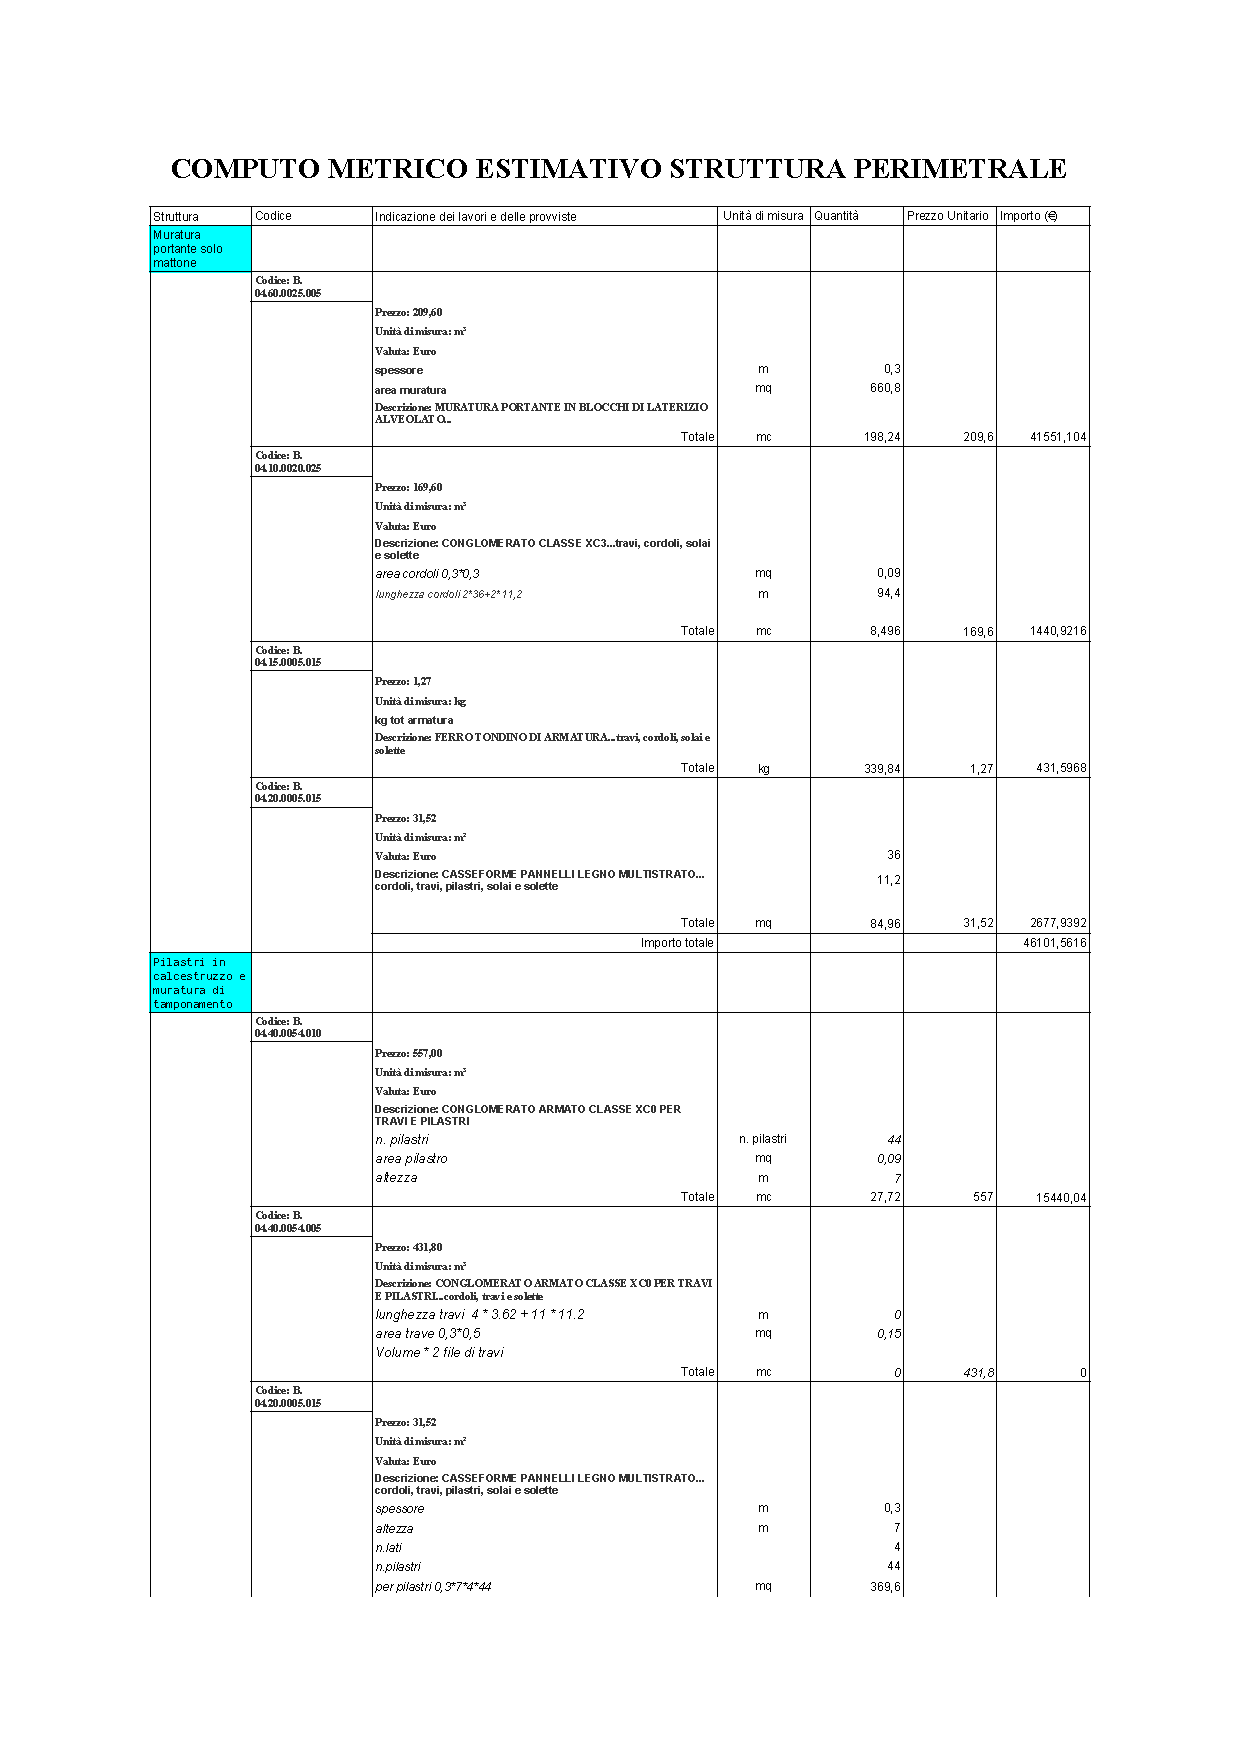
\includepdf[pages={1-3},pagecommand={\thispagestyle{plain}}]{img/STRUTcostoMateriale.pdf}
%Conputo strutture interne e solai:
\label{STRUTMuraturaTotaleIntESol}
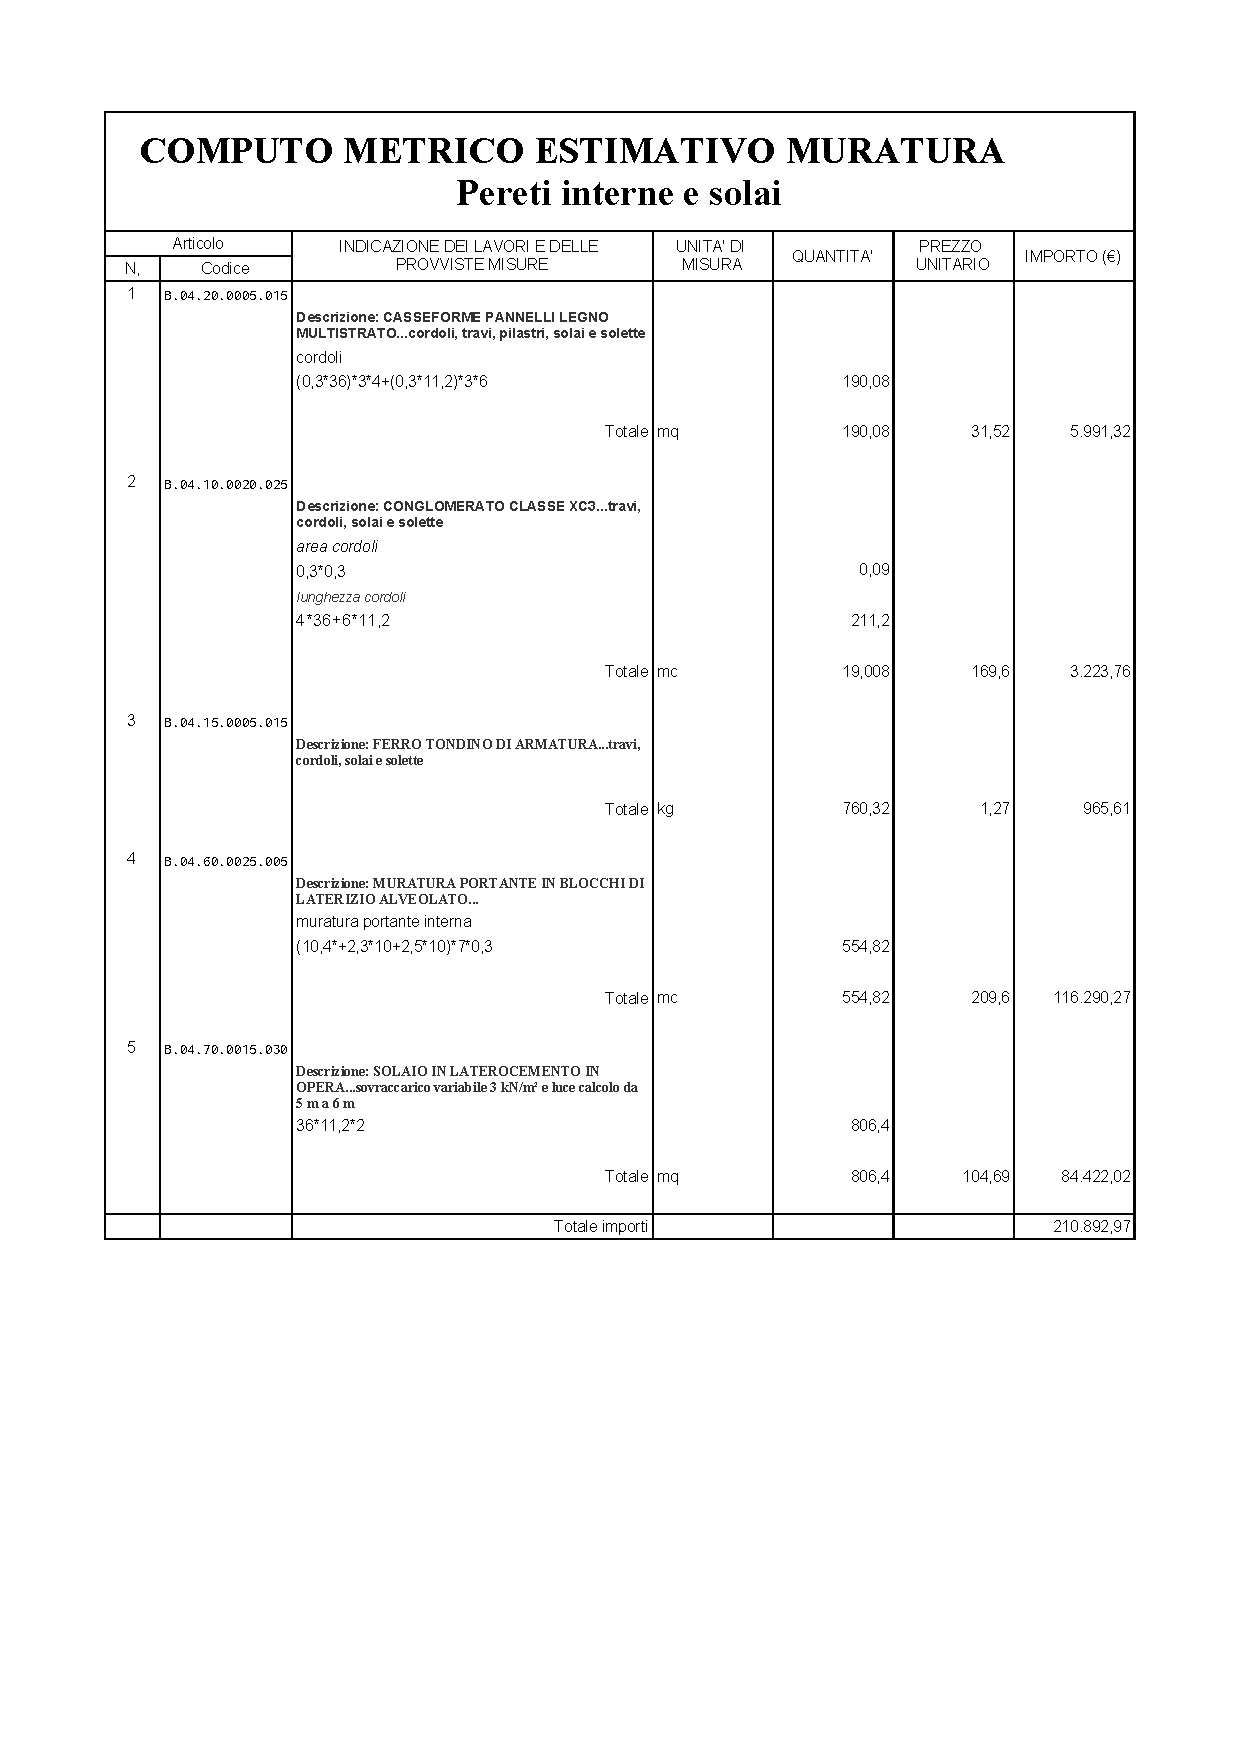
\includepdf[pages={1},pagecommand={\thispagestyle{plain}}]{img/STRUTMuraturaTotaleIntESol.pdf}
%
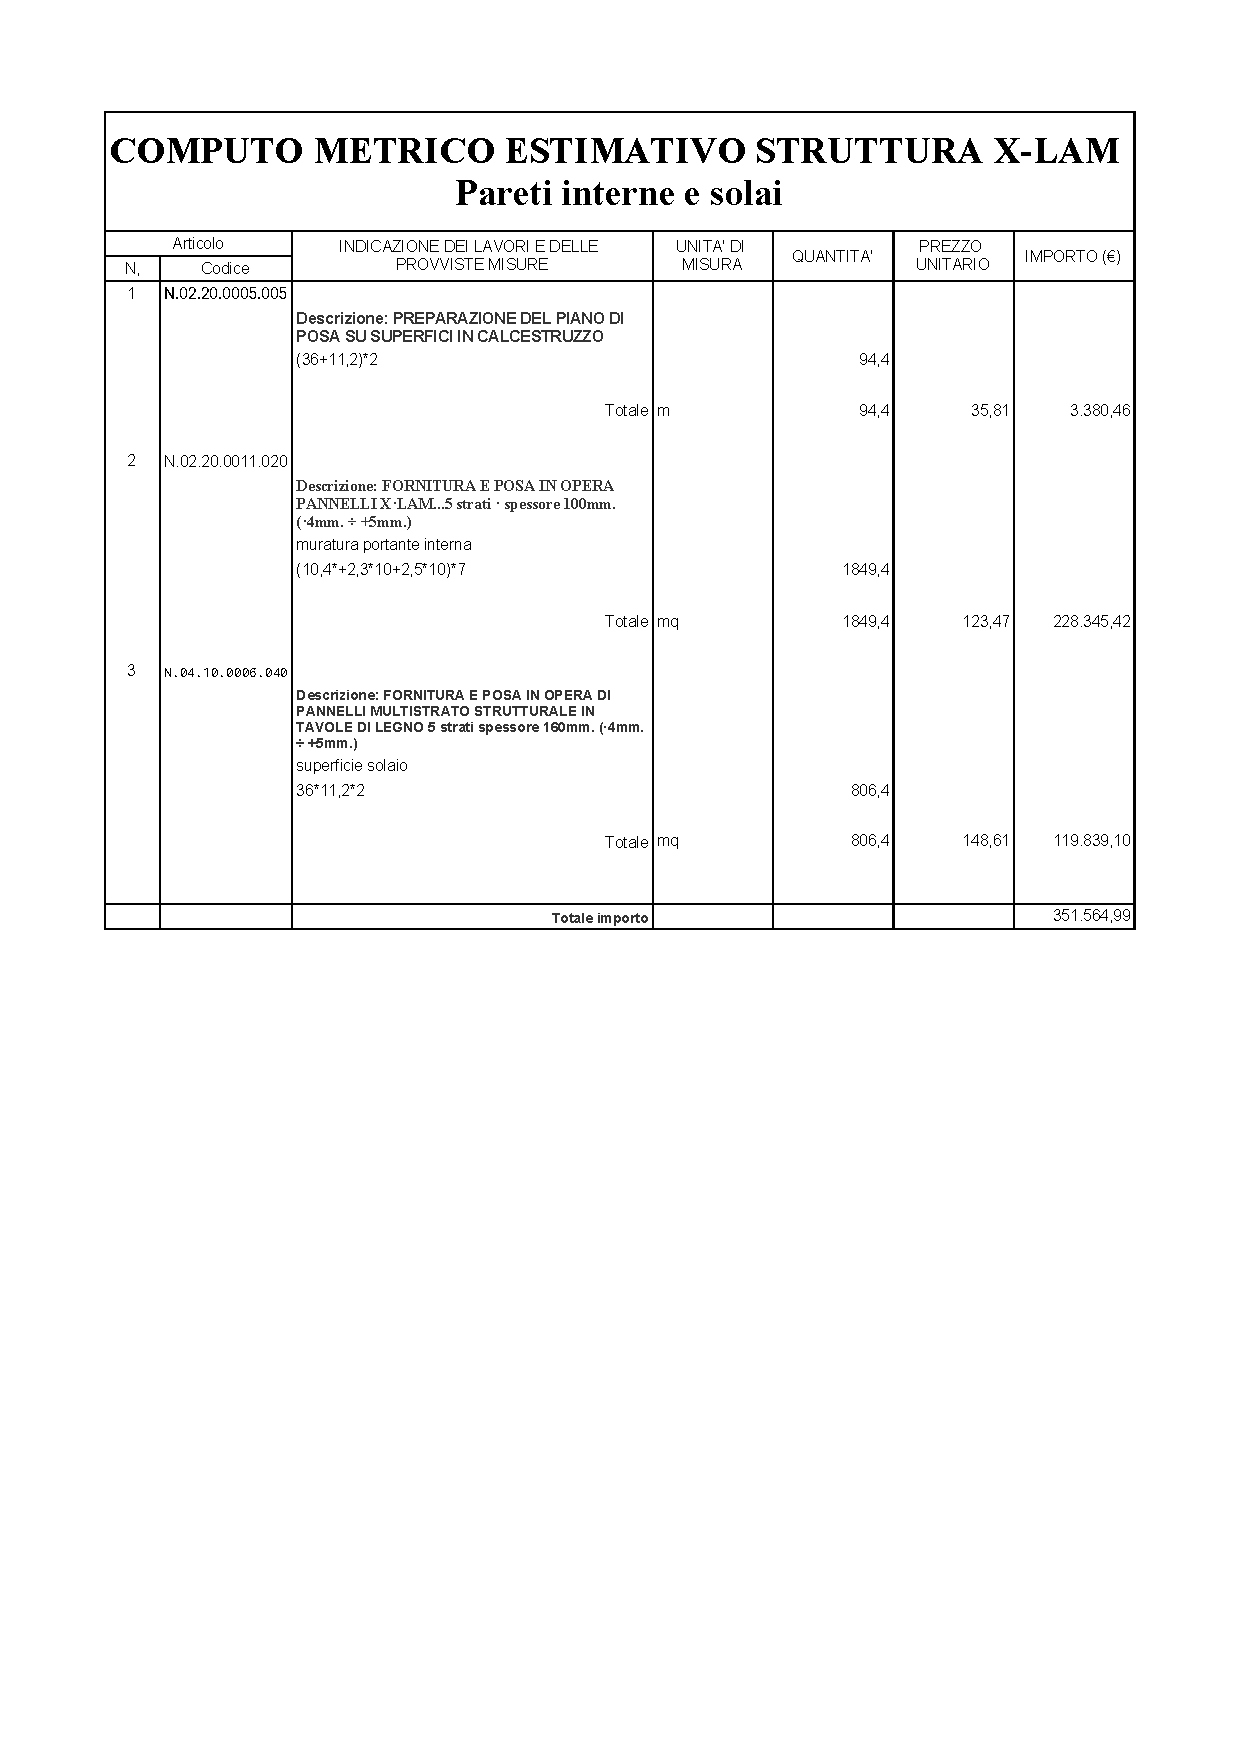
\includepdf[pages={1},pagecommand={\thispagestyle{plain}}]{img/STRUTXLAMTotaleIntESol.pdf}
\end{document}